%%%%%%%%%%%%%%%%%%%%%%%%%%%%%%%%%%%%%%%%%%%%%%%%%%%%%%%%%%%%%%%%%%%%%%%%%%%
%% trime 9.75in x 6.5in
%% Text Area: 8in (include Runningheads) x 5in
%% ws-ijcga.tex   :   19-10-2007
%% Class file to use with ws-ijcga.cls written in Latex2E. 
%% The content, structure, format and layout of this style file is the 
%% property of World Scientific Publishing Co. Pte. Ltd. 
%% Copyright 1995, 2002 by World Scientific Publishing Co. 
%% All rights are reserved.
%%%%%%%%%%%%%%%%%%%%%%%%%%%%%%%%%%%%%%%%%%%%%%%%%%%%%%%%%%%%%%%%%%%%%%%%%%%%
%
\documentclass{ws-ijcga}
\usepackage{amsopn,amsmath}
%\usepackage{hyperref}
\usepackage{graphicx}
\usepackage{url}
\listfiles

\DeclareMathOperator{\cn}{cr}

\newcommand{\const}{268.19}
\newcommand{\R}{\mathbb{R}}

\begin{document}

\markboth{
D. Charlton,
E. D. Demaine,
M. L. Demaine,
V. Dujmovi\'c,
P. Morin, and
R. Uehara}
{Ghost Chimneys}



\catchline

\title{Ghost Chimneys\footnote{Preliminary version was presented at the
22nd Canadian Conference on Computational Geometry.}}

\author{David Charlton\footnote{Supported in part by Akamai Presidential Fellowship.},
Erik D. Demaine,
Martin L. Demaine
}
%
\address{Computer Science and Artificial Intelligence Laboratory, MIT, Cambridge, USA.\\
\protect\url{{dchar,edemaine,mdemaine}@mit.edu}} 

% \author{}
% %
% \address{Computer Science and Artificial Intelligence Laboratory, MIT, Cambridge, USA.\\
% \protect\url{edemaine@mit.edu}} 

% \author{}
% %
% \address{Computer Science and Artificial Intelligence Laboratory, MIT, Cambridge, USA.\\
% \protect\url{mdemaine@mit.edu}} 

\author{Vida Dujmovi\'c\footnote{Research supported in part by NSERC.},
\addtocounter{footnote}{-1}
Pat Morin\footnotemark%{Research supported in part by NSERC.}
}
%
\address{School of Computer Science, Carleton University, Ottawa, Canada.\\
\protect\url{{vida,morin}@scs.carleton.ca}} 

% \author{Pat Morin\footnote{Research supported in part by NSERC.}}
% %
% \address{School of Computer Science, Carleton University, Ottawa, Canada.\\
% \protect\url{morin@scs.carleton.ca}} 

\author{Ryuhei Uehara\footnote{Supported in part by
Ogasawara Foundation for the Promotion of Science and Engineering.}}
%
\address{School of Information Science, JAIST, Ishikawa, Japan.\\
\protect\url{uehara@jaist.ac.jp}} 

\maketitle

\pub{Received (received date)}{Revised (revised date)}
{Communicated by (Name)}

\begin{abstract}
A planar point set $S$ is an $(i,t)$ \emph{set of ghost chimneys}
if there exist lines $H_0,H_1,\ldots,H_{t-1}$ such that the orthogonal
projection of $S$ onto $H_j$ consists of exactly $i+j$ distinct points.
We give upper and lower bounds on the maximum value of $t$
in an $(i,t)$ set of ghost chimneys, showing that it is linear in~$i$.

\keywords{Crossing lemma; orthogonal projection; shadow sculpture.}
\end{abstract}

\section{Introduction}

Once upon a time in Japan, there was a power plant with four chimneys
called ``ghost chimneys'' (obake entotsu, or
\raisebox{-1pt}{
\includegraphics[height=9pt]{obake_entotsu}});
see \figurename~\ref{fig:chimneys}.
Although these chimneys were dismantled in 1964, they are still famous
in Japan, with toys, books, manga, and movies referencing them (\figurename~\ref{fig:kitty}).
%(For example, the web page for the chimneys 
%is still maintained and managed by the city.
They are considered a kind of symbol of industrialized Japan
in the old, good age of the Showa era\cite{adachi}.
%(see \url{http://www.city.adachi.tokyo.jp/003/d10100040.html}); in Japanese!

One of the reasons why they are famous and are called ``ghost chimneys''
is that they could be seen as two chimneys, three chimneys, 
or four chimneys depending on the point of view.
This phenomenon itself was an accident, but it raises several natural questions.
What interval of integers can be realized by such chimneys?
How many chimneys do we need to realize the interval?
How can we arrange the chimneys to realize the interval?

More precisely, we consider the following problem: given an integer $i$, what
is the maximum value $t(i)$ such that there exists a set of points
$S\subset\R^2$ and a set $H_0,H_1,\ldots,H_{t(i)-1}$ of lines where, for each
$j\in\{0,1,\ldots,t(i)-1\}$, the orthogonal projection of $S$ onto $H_j$
consists of exactly $i+j$ distinct points?  We prove the following result:

\begin{theorem}\label{th:main}
For any integer $i\ge 1$,  $2i \le t(i) < 123.33i+1$.
\end{theorem}

In addition to Theorem \ref{th:main}, we show that $t(1)=2$, $t(2)=5$, $t(3)=9$,
and $12\le t(4)\le 15$.  These results show that neither the lower bound
nor the upper bound of Theorem \ref{th:main} is tight for all values of $i$.
Theorem \ref{th:main} is an immediate consequence of Lemma \ref{lem:lower-bound} and
Lemma \ref{lem:upper-bound}, which we prove in the next two sections, respectively.

% \begin{figure}
%   \centering
% %  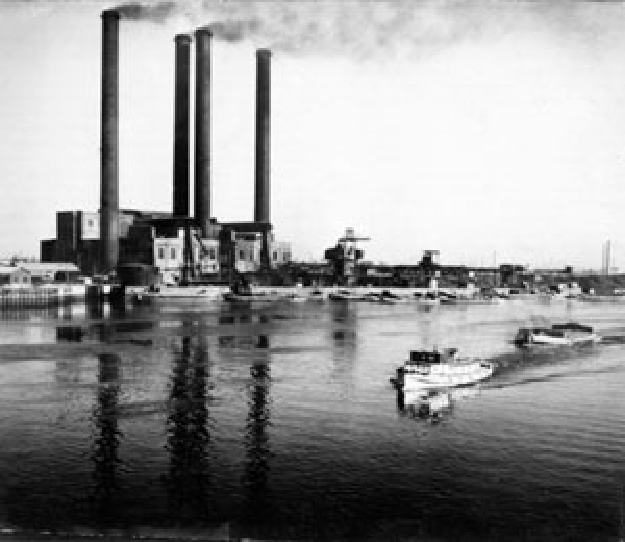
\includegraphics[width=0.85\linewidth]{photo.jpg}
%   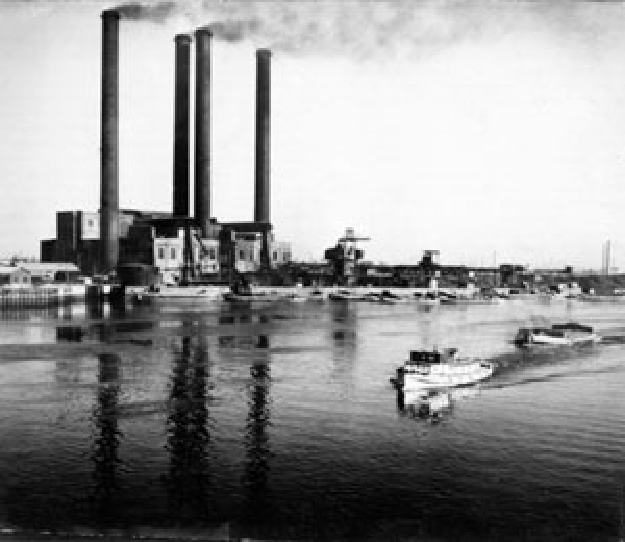
\includegraphics[width=0.45\linewidth]{photo.ps}
%   \caption{The ghost chimneys in Japan, part of the Senju Thermal Power Station
%            (1926--1964) maintained by the Tokyo Electric Power Company.
%            [Used with permission from Adachi City.]}
%   \label{fig:chimneys}
% \end{figure}
% \begin{figure}
%   \centering
% %  
\includegraphics[width=0.85\linewidth]{kitty.jpg}
%   
\includegraphics[width=0.45\linewidth]{kitty.ps}
%   %\caption{Kitty on the ghost chimneys.}
%   \caption{Hello Ghosty}
%   \label{fig:kitty}
% \end{figure}

\begin{figure}
  \centering
\begin{minipage}[t]{0.47\textwidth}
  \centering
  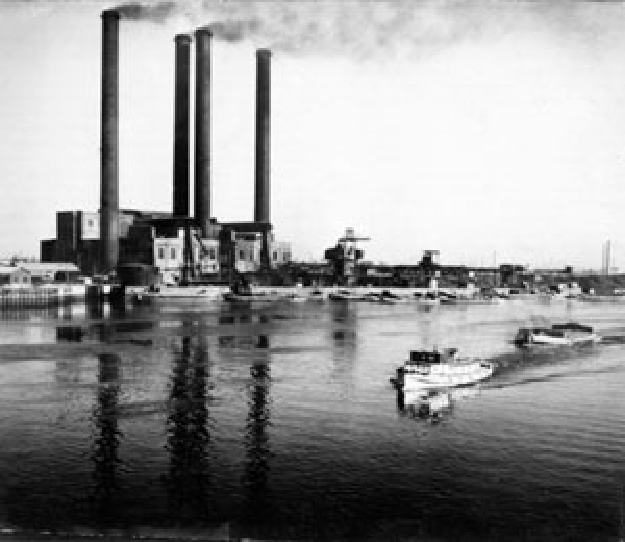
\includegraphics[width=1\linewidth]{photo}
  %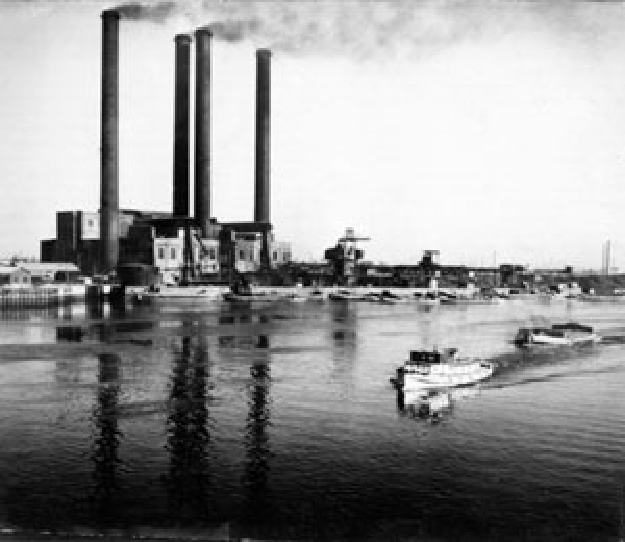
\includegraphics{photo}
  \caption{The ghost chimneys in Japan, part of the Senju Thermal Power Station
           (1926--1964) maintained by the Tokyo Electric Power Company.
           [Used with permission from Adachi City.]}
  \label{fig:chimneys}
\end{minipage}
\hfil
\begin{minipage}[t]{0.47\textwidth}
  \centering
  
\includegraphics[width=1\linewidth]{kitty}
  \caption{Hello Kitty Obake-Entotsu version (\copyright{} 1976, 2011 SANRIO CO.,LTD.~APPROVAL NO.~S520196)}
  \label{fig:kitty}
\end{minipage}
\end{figure}

These ghost-chimney problems relate more generally to understanding
what orthogonal projections a single 2D or 3D shape can have. In 2D,
some closely related problems have been considered\cite{Ski,mat}. 
Past explorations into structures in 3D, known variously as 3D ambigrams,
trip-lets, and shadow sculptures, have focused on precise, usually
connected projections\cite{triplets,ShadowArt}. 
Our work was originally motivated by considering what happens with disconnected projections of unspecified relative position.

\section{The Lower Bound}
\begin{figure*}
  \centering
  \begin{tabular}{cc}
%    & 
\includegraphics[scale=0.9,bb=217 234 389 309]{j0.pdf} \\ 
%     & 
\includegraphics[scale=0.9]{j0.ps} \\ 
%     & $j = 0$  \\
\multicolumn{2}{c}{
\includegraphics[scale=0.9]{j0}}\\
\multicolumn{2}{c}{$j=0$}\\
%     
\includegraphics[scale=0.9,bb=217 234 389 309]{j1.pdf} & 
%     
\includegraphics[scale=0.9,bb=217 234 389 309]{j2.pdf} \\
     
\includegraphics[scale=0.9]{j1} & 
     
\includegraphics[scale=0.9]{j2} \\
      $j=1$ & $j=2$ \\
%     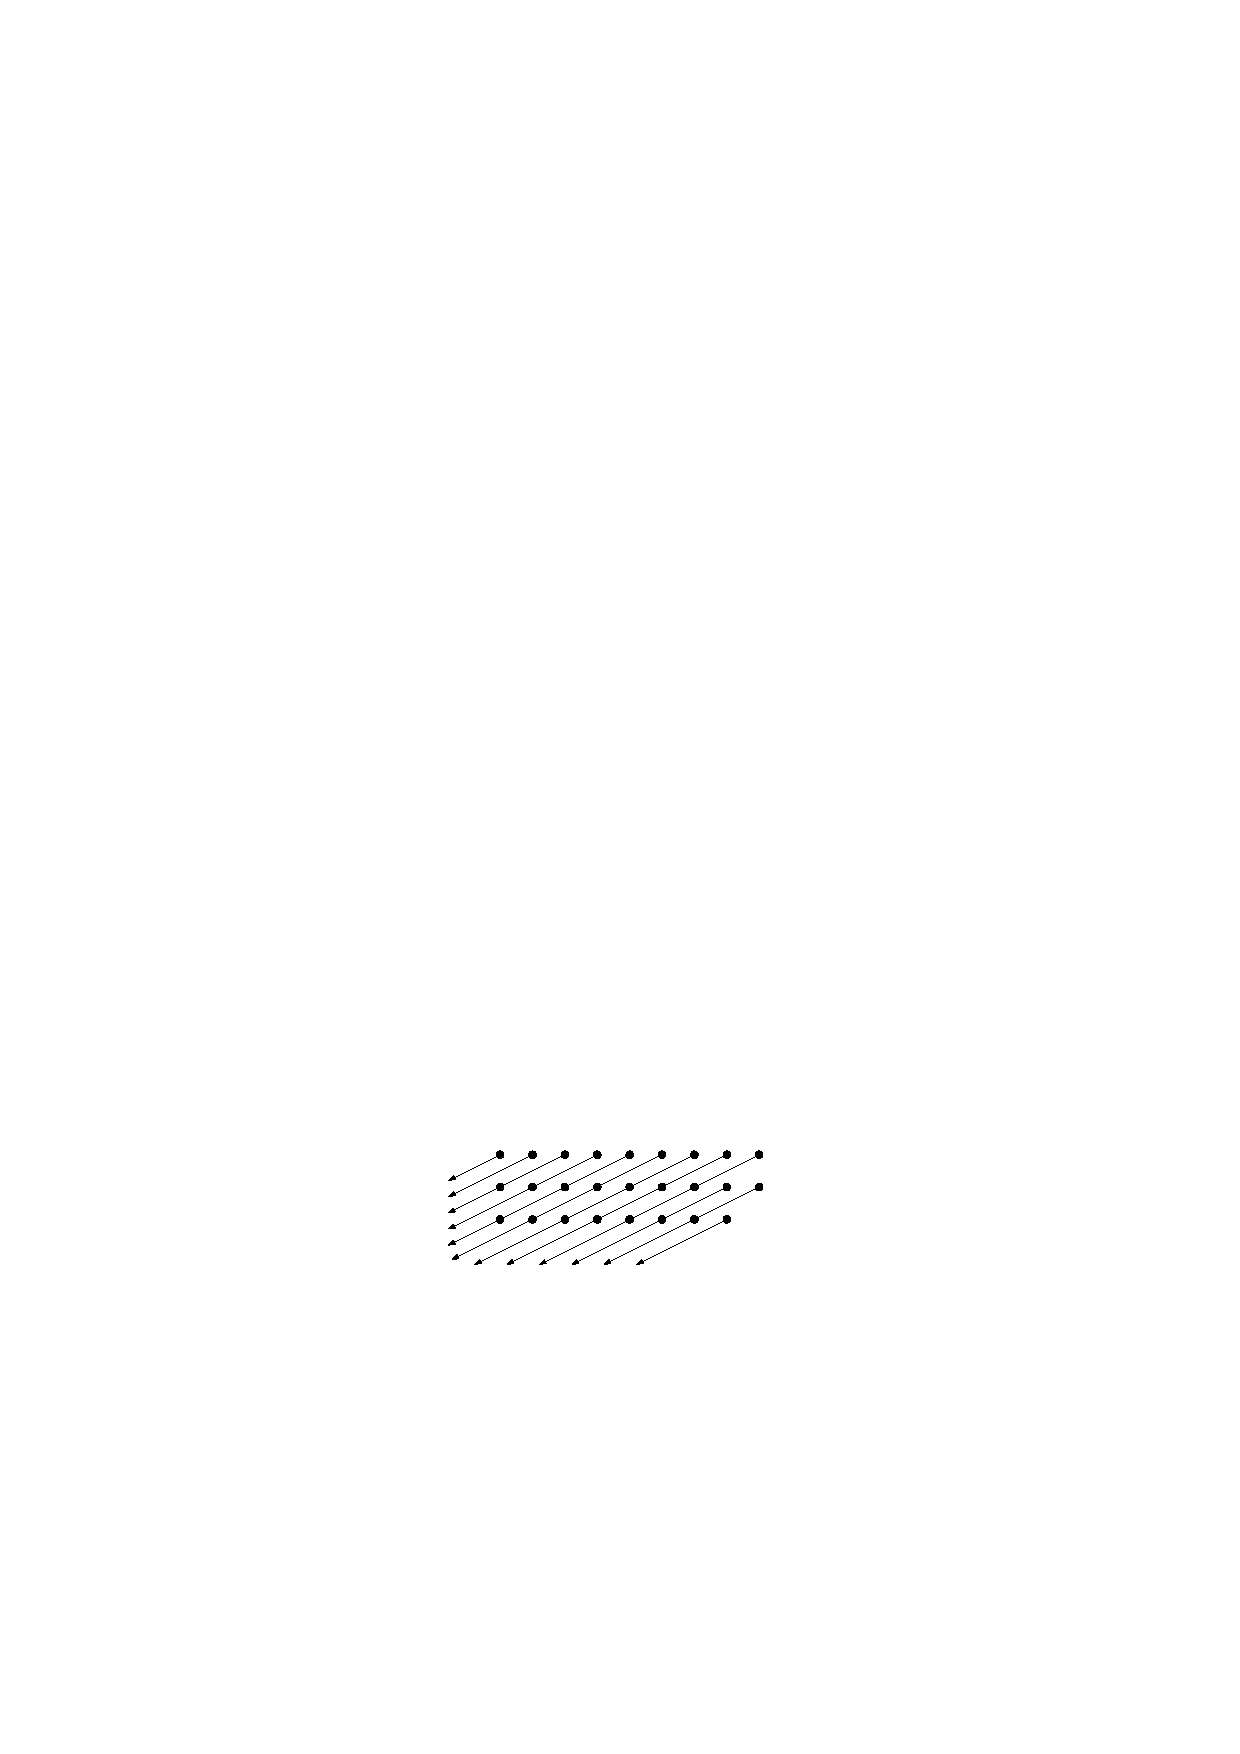
\includegraphics[scale=0.9,bb=215 234 389 309]{j3.pdf} & 
%     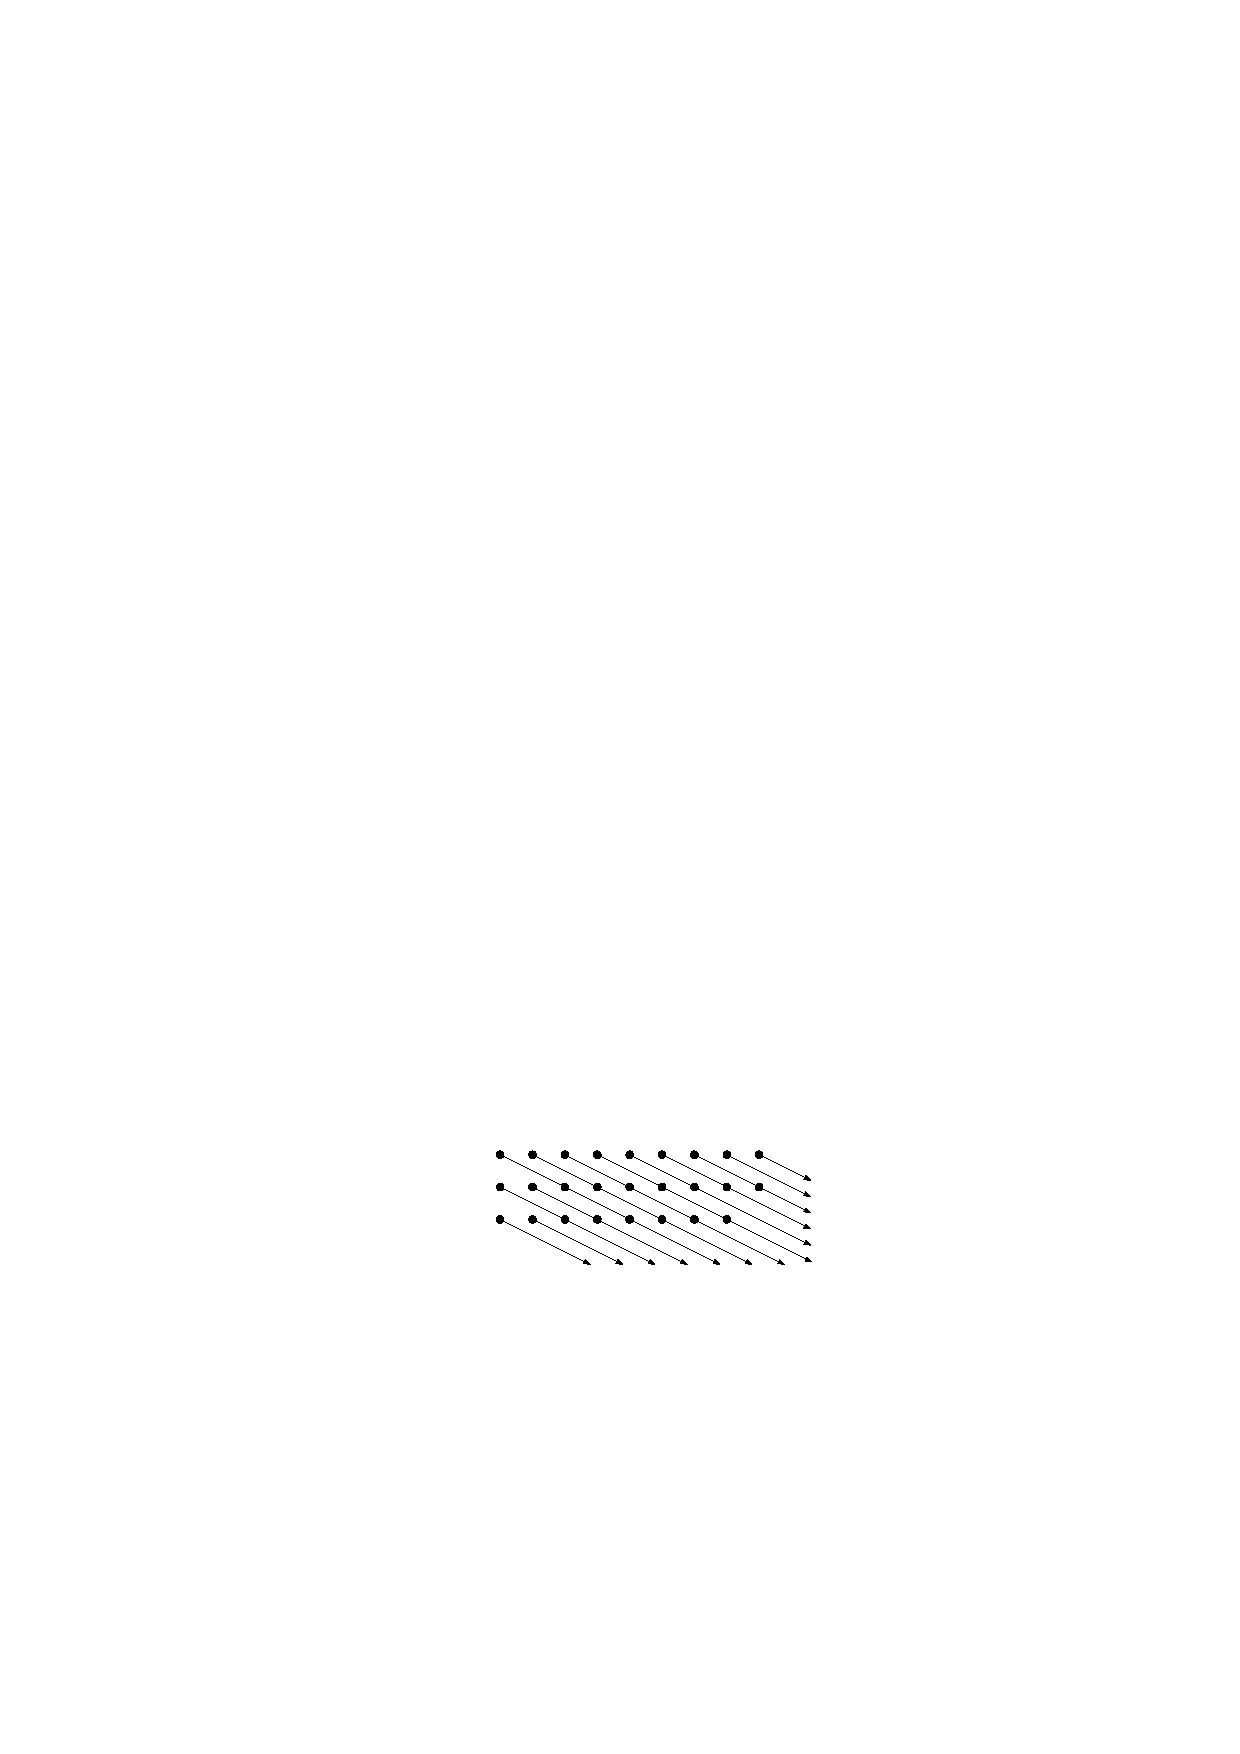
\includegraphics[scale=0.9,bb=217 234 390 309]{j4.pdf} \\
     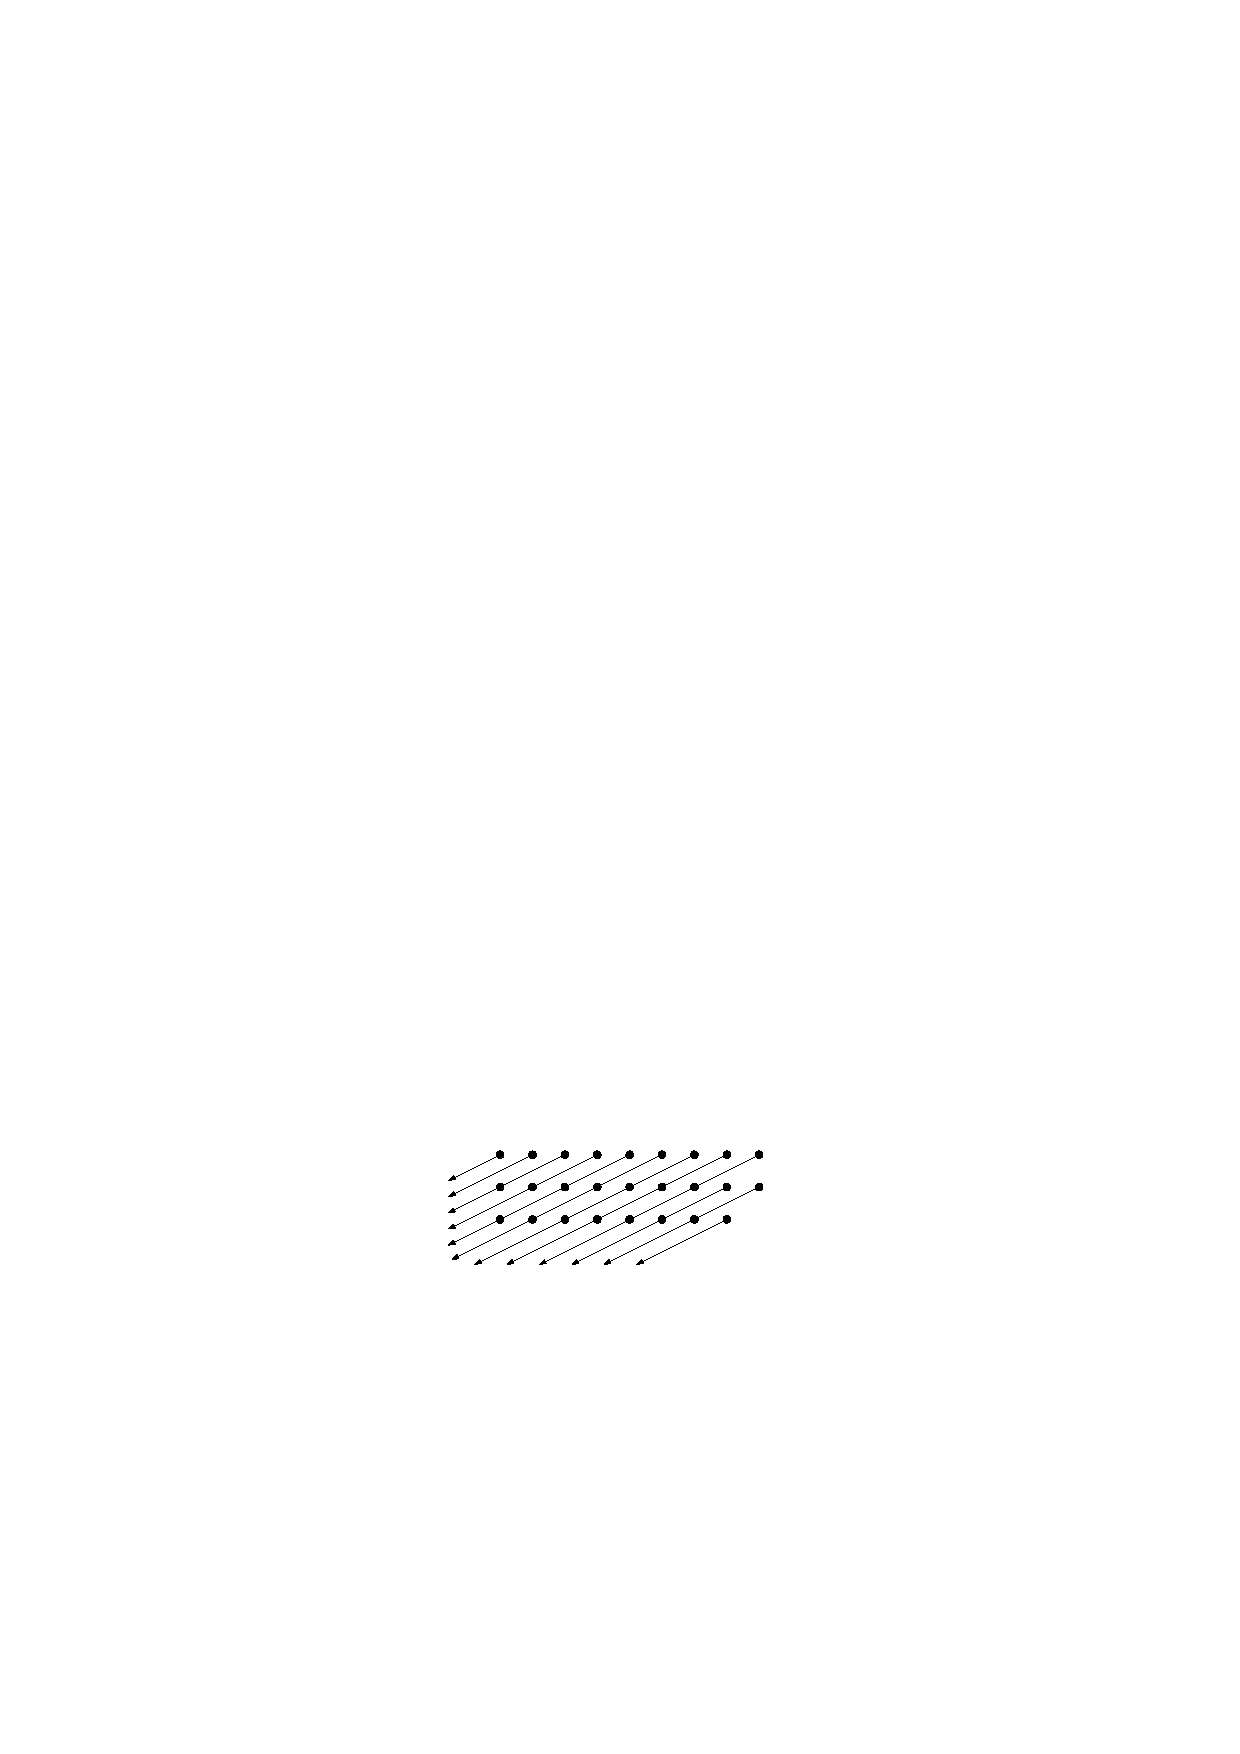
\includegraphics[scale=0.9]{j3} & 
     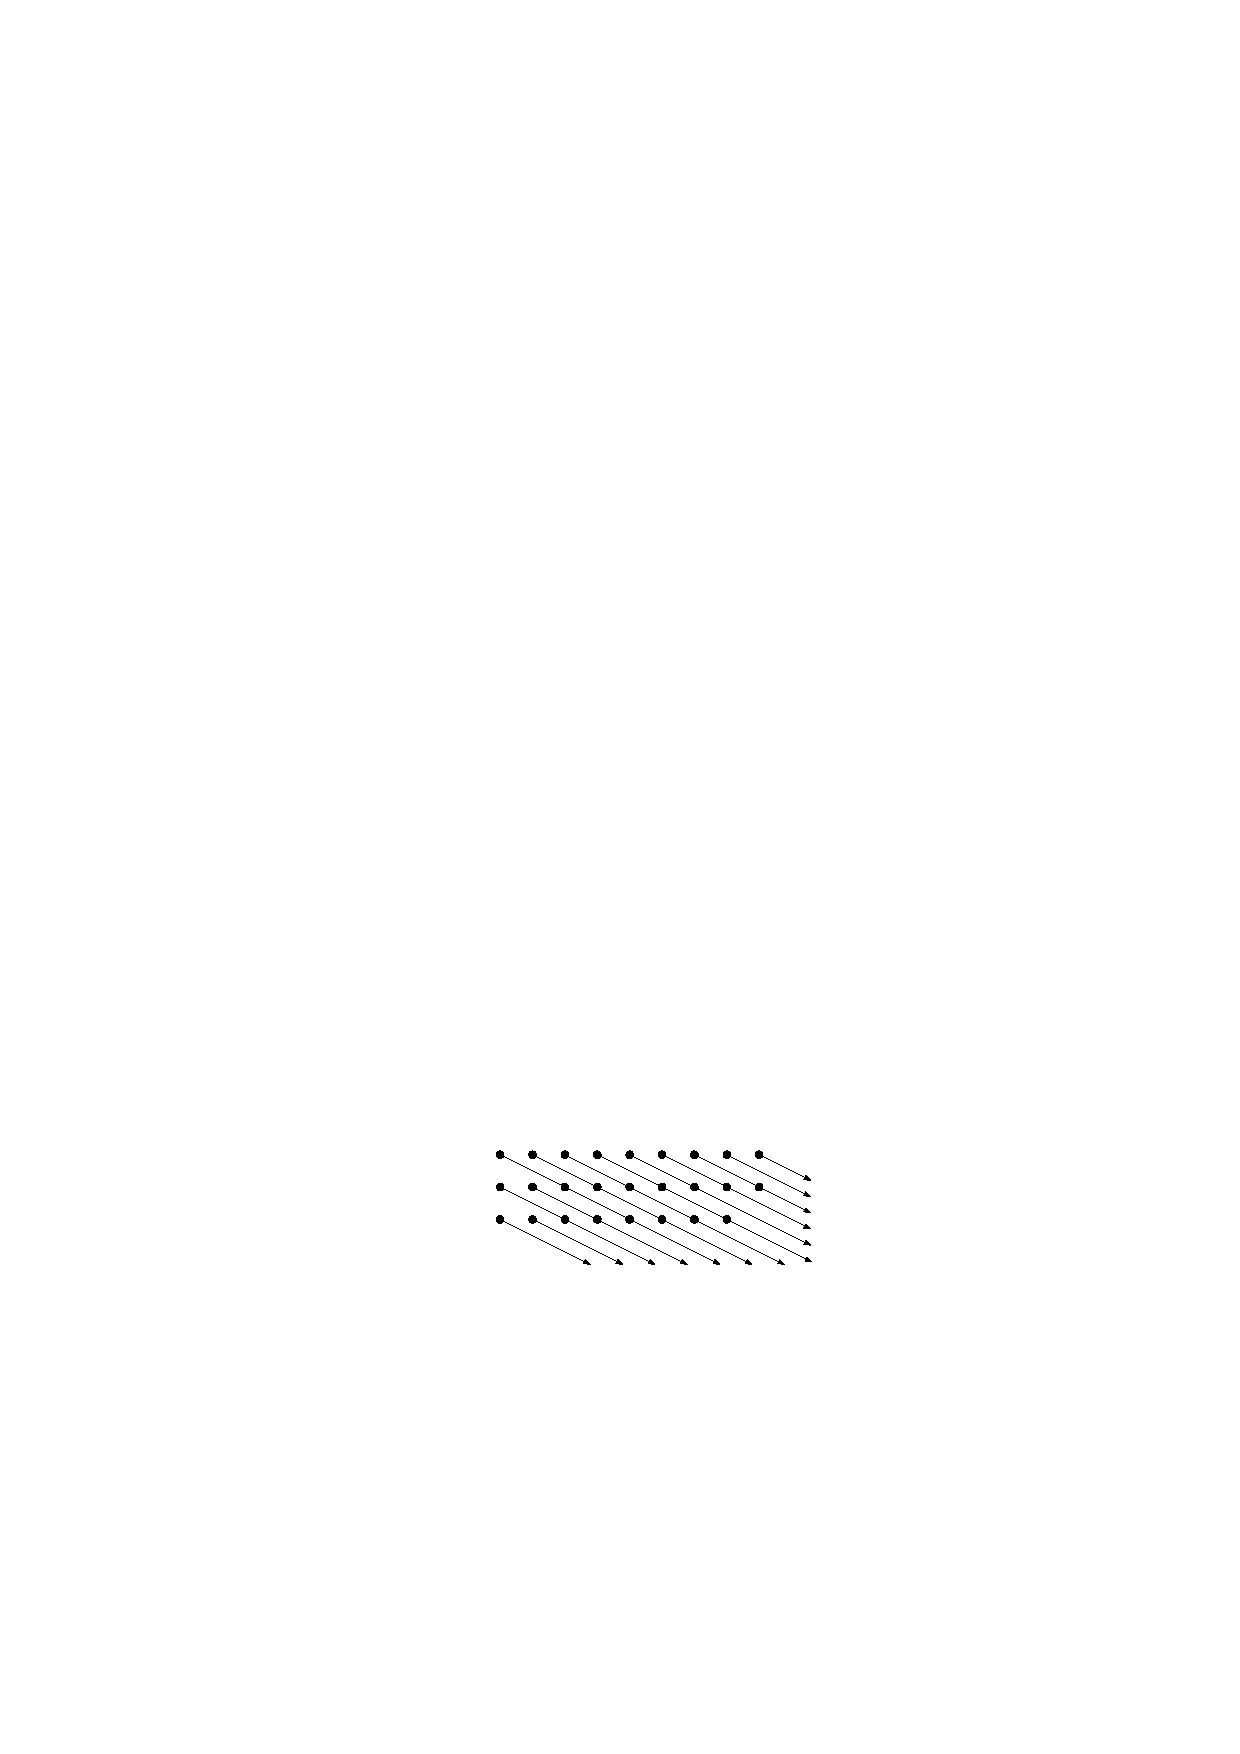
\includegraphics[scale=0.9]{j4} \\
      $j=3$ & $j=4$
  \end{tabular}
  \caption{The set $S(i)$  for $i=9$ and the projection directions that yield $i,i+1,\ldots,i+4$ distinct points.}
  \label{fig:lower-bound}
\end{figure*}


\begin{lemma}\label{lem:lower-bound}
For each integer $i\ge 1$, there exists a set $S=S(i)$ of $3i-1$
points and a set $H_0,H_1,\ldots,H_{2i-1}$ of lines such that, for each
$j\in\{0,1,\ldots,2i-1\}$, the orthogonal projection of $S$ onto $H_j$
has exactly $i+j$ distinct values.
\end{lemma}

\begin{proof}
The point set $S$ consists of the points of an $i\times 3$ grid with the bottom-right corner removed; see \figurename~\ref{fig:lower-bound}.  For even $j$, $H_j$ is a line of slope $j/2$.  For odd~$j$, $H_j$ is a line of slope $-(j+1)/2$.
\end{proof}



\section{The Upper Bound}

Our upper-bound proof is closely related to Sz\'ekely's proof of the
Szem\'eredi-Trotter Theorem\cite{s97}.  We make use of the following
version of the Crossing Lemma, which was proved by Pach, Radoi\v{c}i\'{c},
Tardos, and T\'oth\cite{prtt04}:

\begin{lemma}[Crossing Lemma]\label{lem:crossing}
Let
$\beta=103/6$, $\gamma = 1024/31827$, and let
$G$ be a graph with no self loops, no parallel edges, $v$ vertices, and
$e > \beta v$ edges.  
Then the crossing number $\cn(G)$, the minimum number of edge crossings
 in a certain drawing of $G$, is given by
\[
  \cn(G) \ge \gamma \cdot \frac{e^3}{v^2}.
\]
\end{lemma}


\begin{lemma}\label{lem:upper-bound-general}
Let % $t=\alpha i$, let 
$S$ be a set of $r$ points, and let
$H_0,H_1,\ldots,H_{t-1}$ be a set of lines such that the orthogonal projection
of $S$ onto $H_{j}$ gives exactly $i+j$ distinct values.  
Then, $t\le 34$ or $r\le (2i/t + 2 + t/2i)  i/\gamma$.
\end{lemma}

\begin{proof}
Each projection direction $H_j$ defines a set $L_j$ of $i+j$ parallel
lines, each of which contains at least one point of $S$.  Let $G$ be
the geometric graph that contains the points in $S$ plus $t$ additional
points $p_0,p_1,\ldots,p_{t-1}$.  Two vertices in $S$ are connected by an
edge in $G$ if and only if they occur consecutively on some line in
$L=\bigcup_{j=0}^{t-1}L_j$.  Additionally, each vertex $p_j$ is connected
to each of the $i+j$ lexically largest points on each of the
lines in $L_j$.  See \figurename~\ref{fig:graph}.

\begin{figure}
  \begin{center}
%    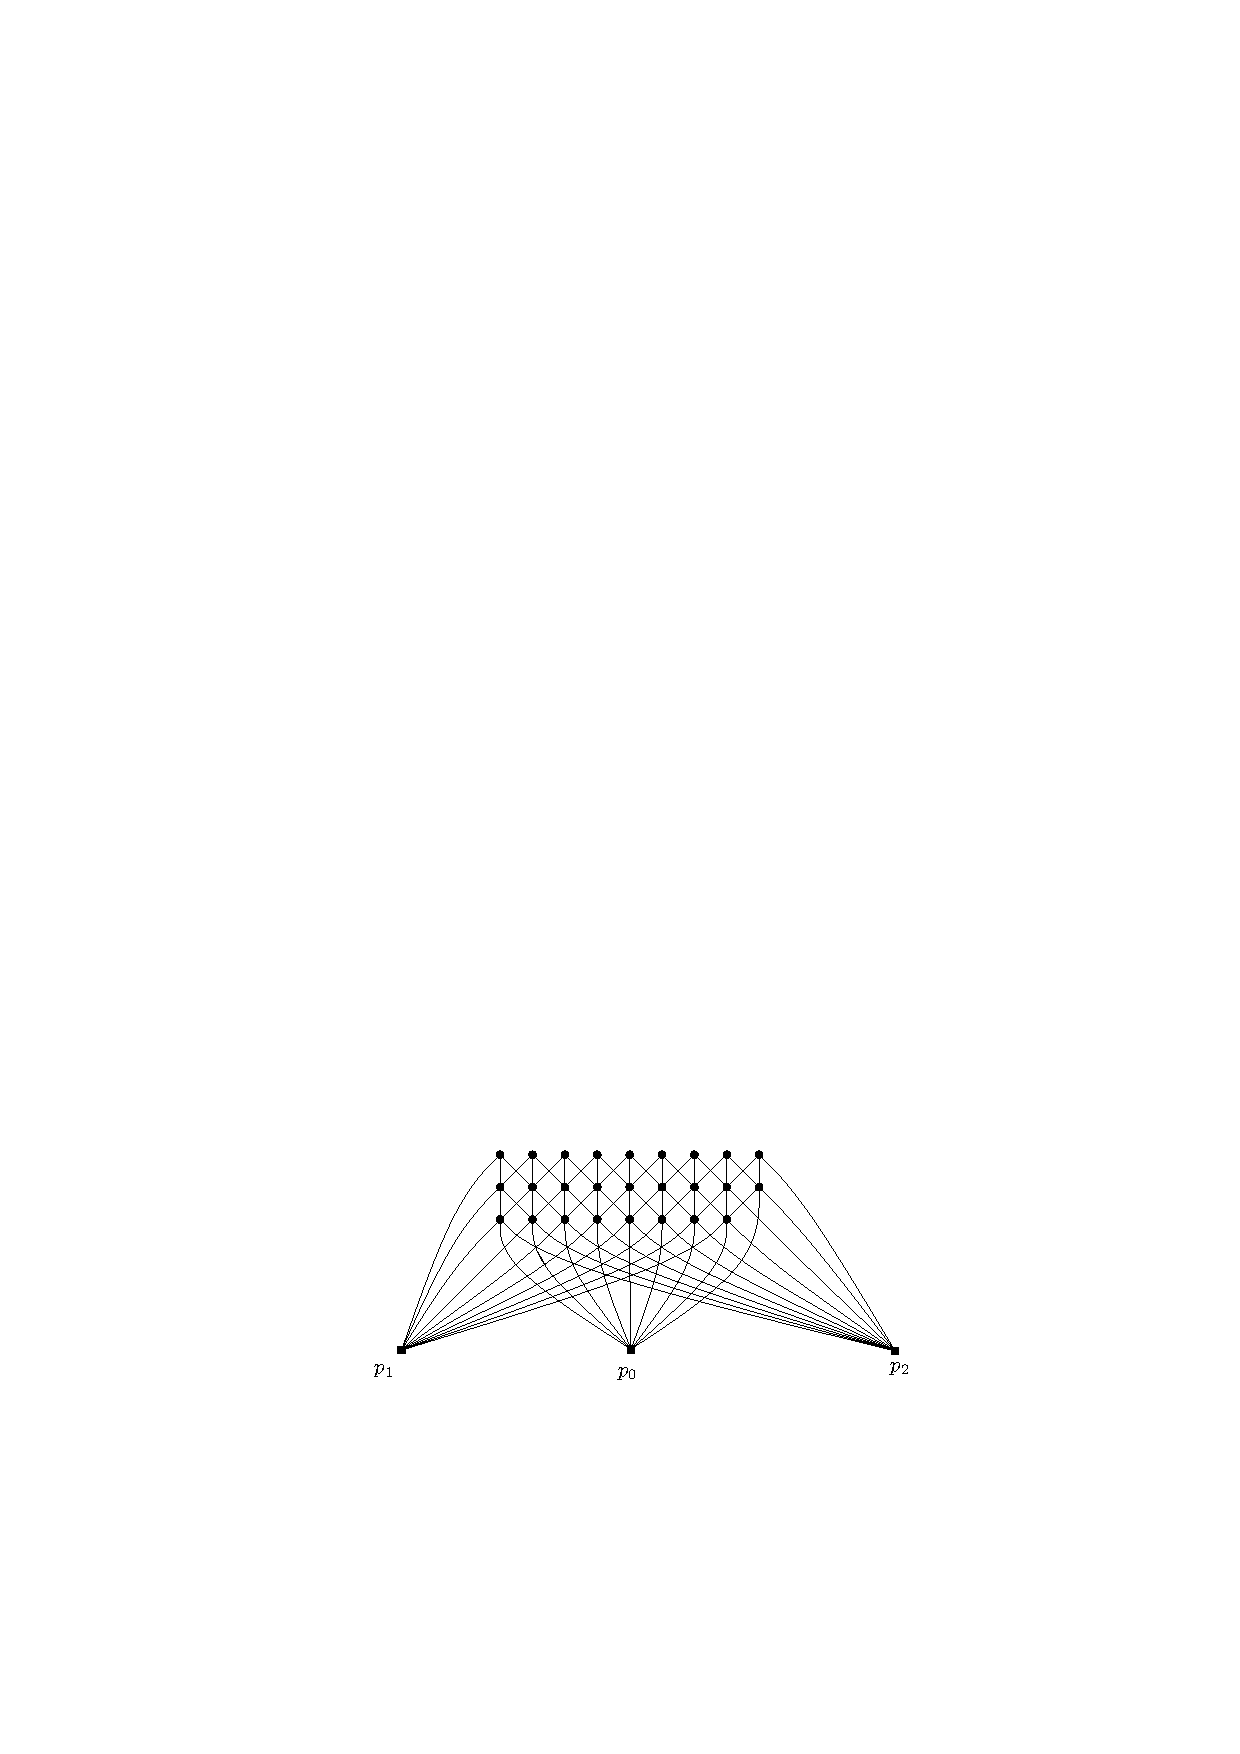
\includegraphics[bb=239 209 439 309]{graph.pdf}
    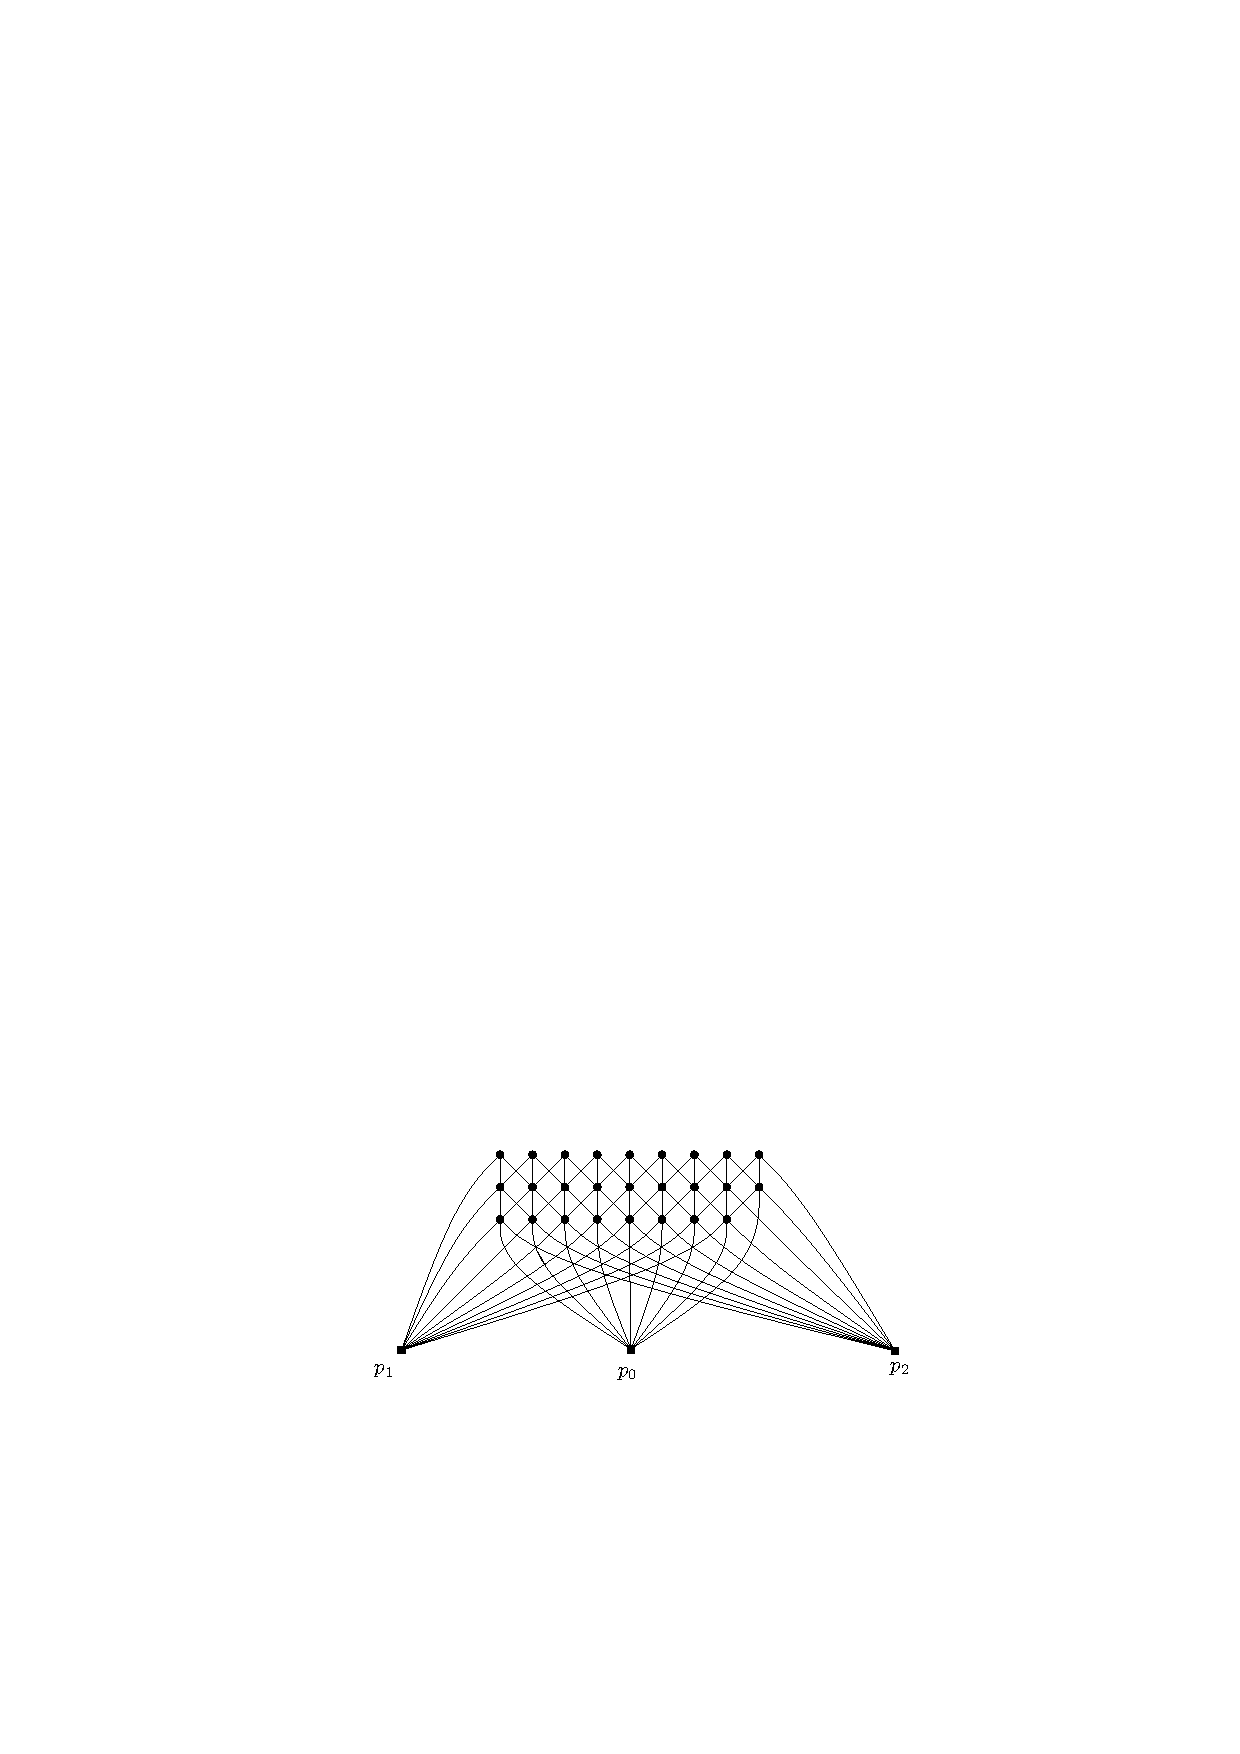
\includegraphics{graph}
  \end{center}
  \caption{The graph $G$ for a set of points with $i=9$ and $t=3$.}
  \label{fig:graph}
\end{figure}

The graph $G$ has $t+r$ vertices
and $tr$ edges.  Observe that we have a drawing of $G$ so that the only
crossings between edges occur where lines in $L$ intersect each other.
The total number $X$ of intersecting pairs of lines in $L$ is
\[
  \begin{aligned}
    X 
      & \le \sum_{j=1}^{t-1}(i+j)\cdot\sum_{k=0}^{j-1}(i+k)
       \le \sum_{j=1}^{t-1}(i+j)(ij + j^2/2) \\
      & \le \sum_{j=1}^{t-1}(i^2j+3ij^2/2 + j^3/2) 
       \le i^2t^2/2 + it^3/2 + t^4/8.
  \end{aligned}
\]

Applying Lemma \ref{lem:crossing}, we learn that either
\begin{equation}
   tr \le \beta (t+r), \label{eq:crossing-a}
\end{equation}
or
\begin{equation}
   X \ge \cn(G) \ge \gamma \frac{(tr)^3}{(t+r)^2} \label{eq:crossing-b}.
\end{equation}

In the former case, we rewrite (\ref{eq:crossing-a}) to obtain
\[
   t \le \beta(t/r + 1) \le 2\beta \le 34 + 1/3,
\]
hence $t\le 34$ (since $t$ is an integer).

In the latter case, we expand (\ref{eq:crossing-b}) to obtain
\[ i^2t^2/2 + it^3/2 + t^4/8 \ge \gamma\frac{(tr)^3}{(t+r)^2} .  \]
Thus
\[ i\left(\frac{i}{2t} 
    + \frac{1}{2}+\frac{t}{8i}\right) 
      \ge \gamma \frac{r^3}{(t+r)^2} \ge \gamma r/ 4,
\]
where the second inequality follows from the fact that $t\le i+t-1 \le r$.
Rewriting to isolate $r$ finally gives
\[
  r \le \left(\frac{2i}{t} + 2 +\frac{t}{2i}\right)i/\gamma,
\]
which completes the proof.
% We finish the proof by observing that, for $\alpha > 2$, the inequality
% $r\le 4i/\gamma$ obtained by setting $\alpha=2$ is stronger and still
% applies.
\end{proof}


\begin{lemma}\label{lem:upper-bound}
For all integers $i\ge 1$, $t(i) < 123.33i+1$.
\end{lemma}

\begin{proof}
The existence of $H_0$ and $H_1$ implies that the points of $S$ lie on 
the intersection of $i$ parallel lines with another set of $i+1$ parallel lines.
Thus, $|S|\le i(i+1)$, so $t(i) \le |S|-i+1\le i^2+1$.
Using this inequality $t(i)\le i^2+1$, the lemma follows for $1\le i\le 123$.
% For $i\in\{1,2,\ldots,17\}$,  by % setting $\alpha = 35/i$.

We assume that $i>123$.  By Lemma \ref{lem:upper-bound-general},
we have $t\le 34$ or $r\le (2i/t + 2 + t/2i)  i/\gamma$.  When $t\le
34$, we are done, so suppose $t>34$.  Notice that, if the conditions of
Lemma~\ref{lem:upper-bound-general} hold for $t$, then they also hold for
all values $t'\in\{35,\ldots,t\}$.  Therefore the statement $r\le (2i/t'
+ 2 + t'/2i) i/\gamma$ is true for all $35\le t'\le t$.  If $t\le 2i$,
then we are done.  Otherwise, taking $t'=2i$ yields
\[
  r\le (2i/t' + 2 + t'/2i) i/\gamma \le 4i/\gamma \enspace .
\]
Combining this with $i+t-1\le r$, we have $i+t-1\le 4i/\gamma$, or $t< 123.33i+1$.

%Therefore, for $i\ge 18$, the lemma follows by applying 
%Lemma \ref{lem:upper-bound-general} with $t/i=2$,
%which gives the minimum value of the function $(2i/t + 2 + t/2i)$. %$\alpha=2$.
% For $i\in\{1,2,\ldots,17\}$, the lemma follows by % setting $\alpha = 35/i$.
% using the inequality $t(i)\le i^2+1$ proven in the next section.
\end{proof}


\section[Small Values of $i$]{\boldmath Small Values of $i$}

In this section we give some tighter bounds on $t(i)$ for
$i\in\{1,2,3,4\}$.

\begin{lemma}\label{lem:i1i2}
$t(1) = 2$, and $t(2)=5$.
\end{lemma}

\begin{proof}
Point sets achieving these bounds are the $1\times 2$ and the $2\times 3$
grid, respectively; see \figurename~\ref{fig:i1i2}.  
That these point sets are optimal follows from the inequality $t(i)\le i^2+1$ 
shown in the proof of Lemma \ref{lem:upper-bound}.
\end{proof}

\begin{figure}
  \centering
  \begin{tabular}{cc}
%     \hspace{-0.5in}
%      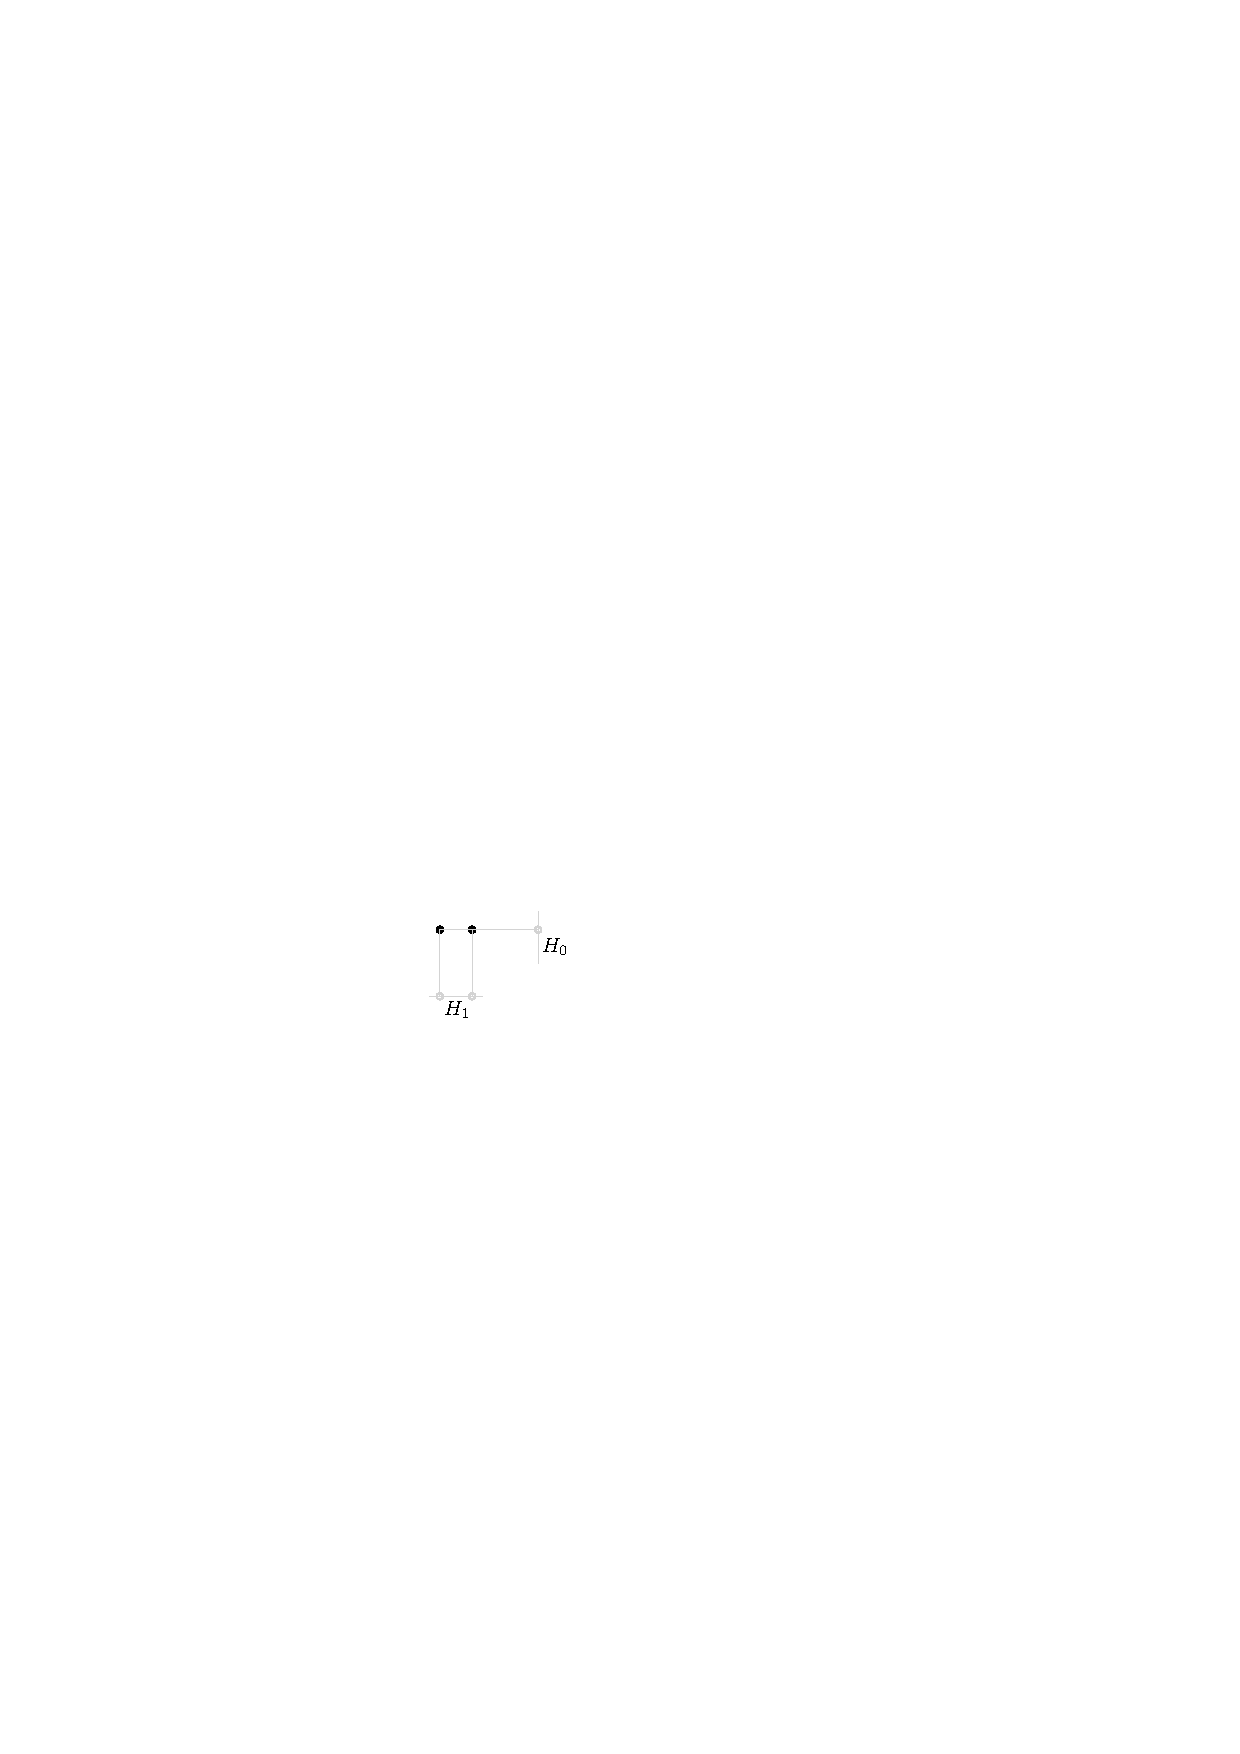
\includegraphics[bb=170 335 283 417]{i1.pdf} & 
%      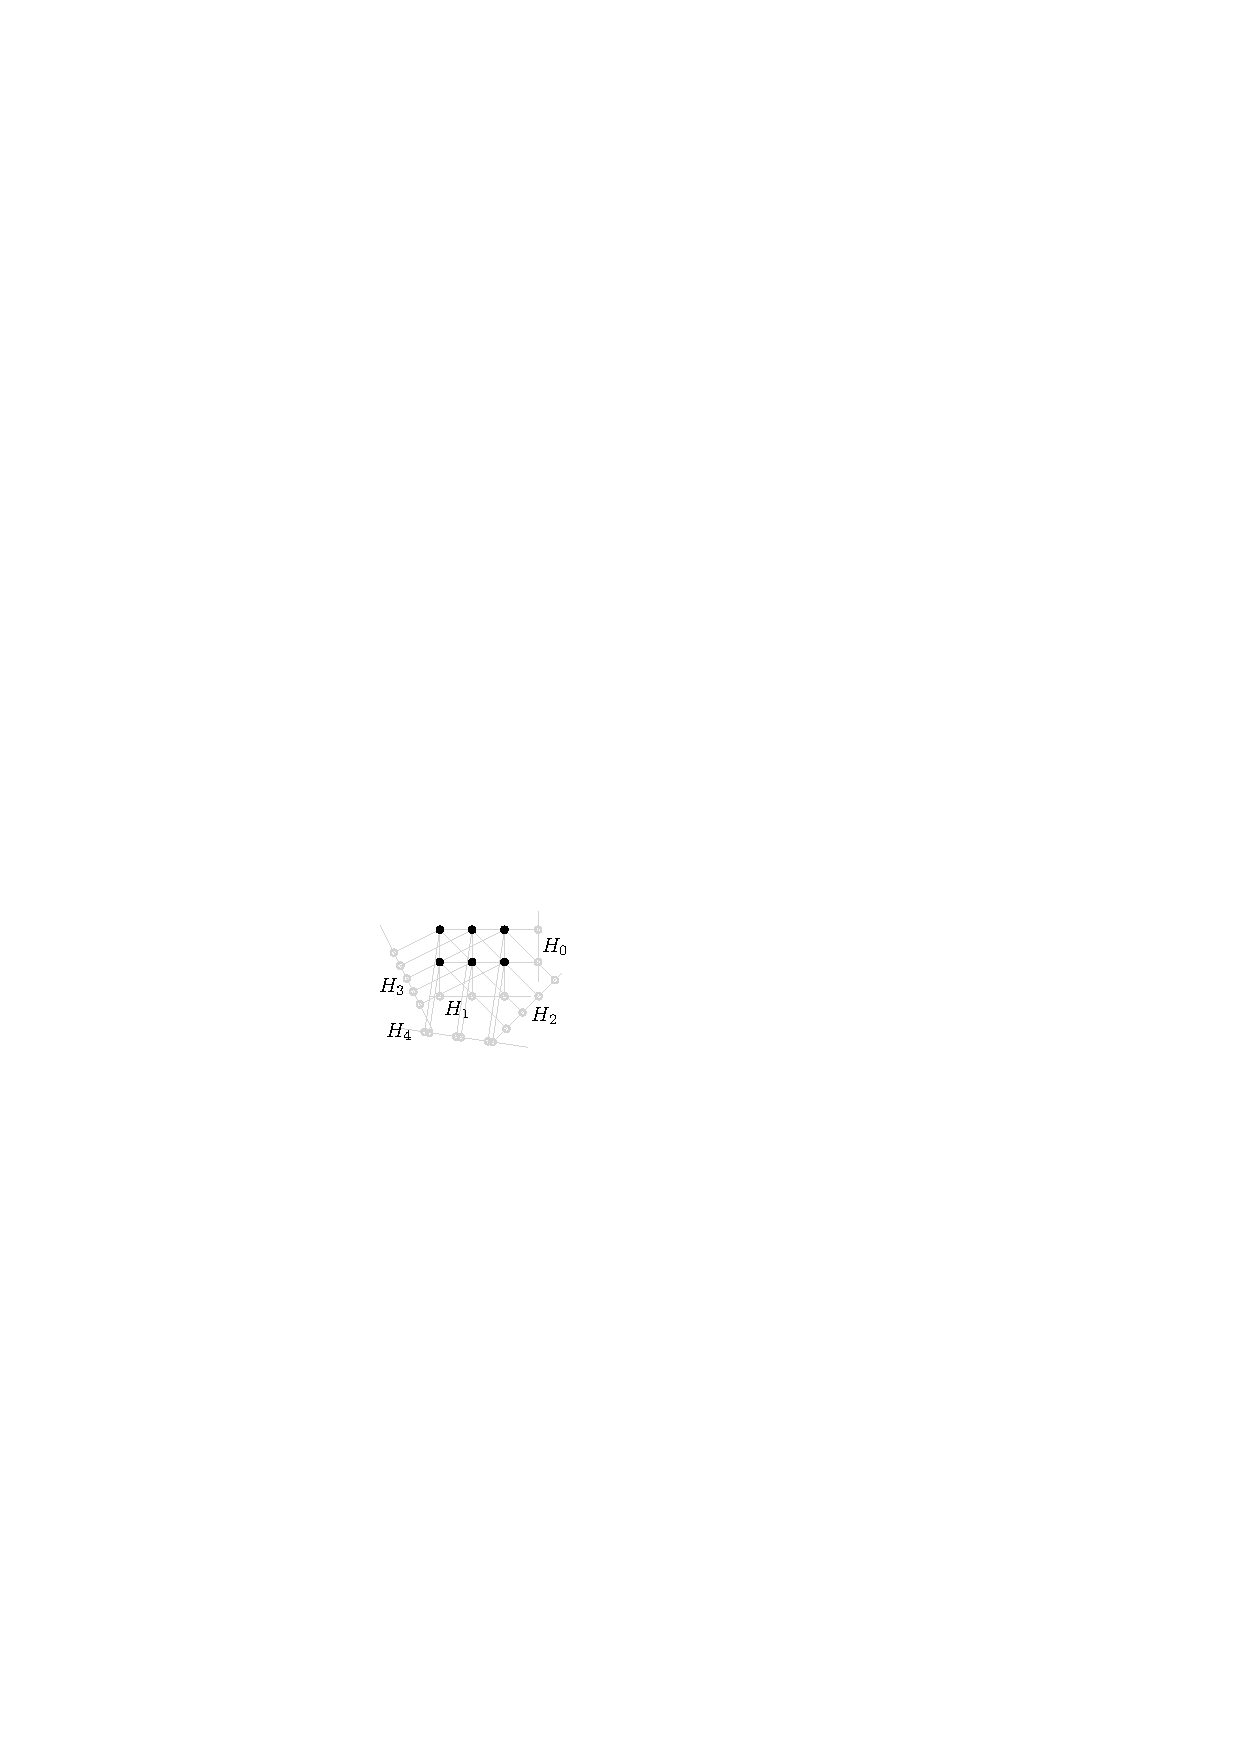
\includegraphics[bb=170 335 283 417]{i2.pdf} \\
      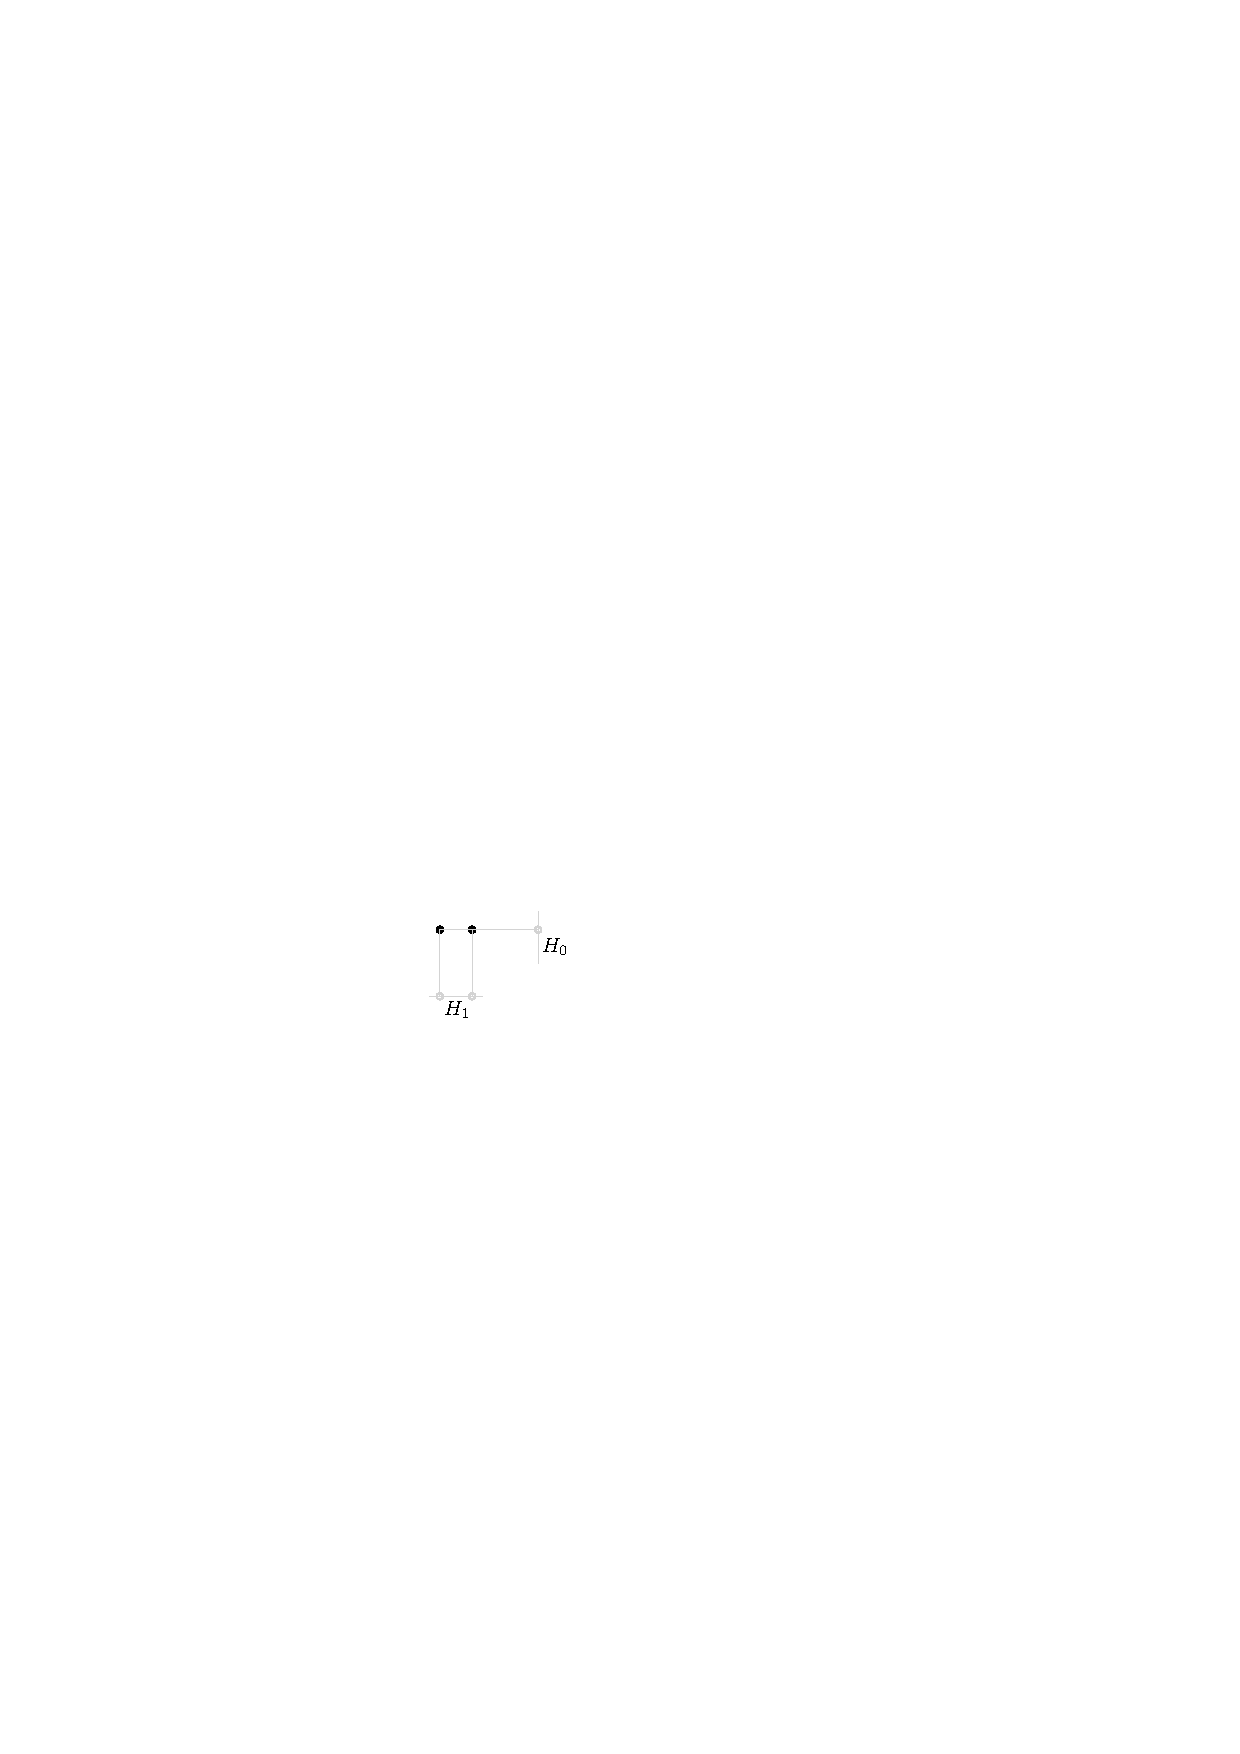
\includegraphics{i1.pdf} & 
      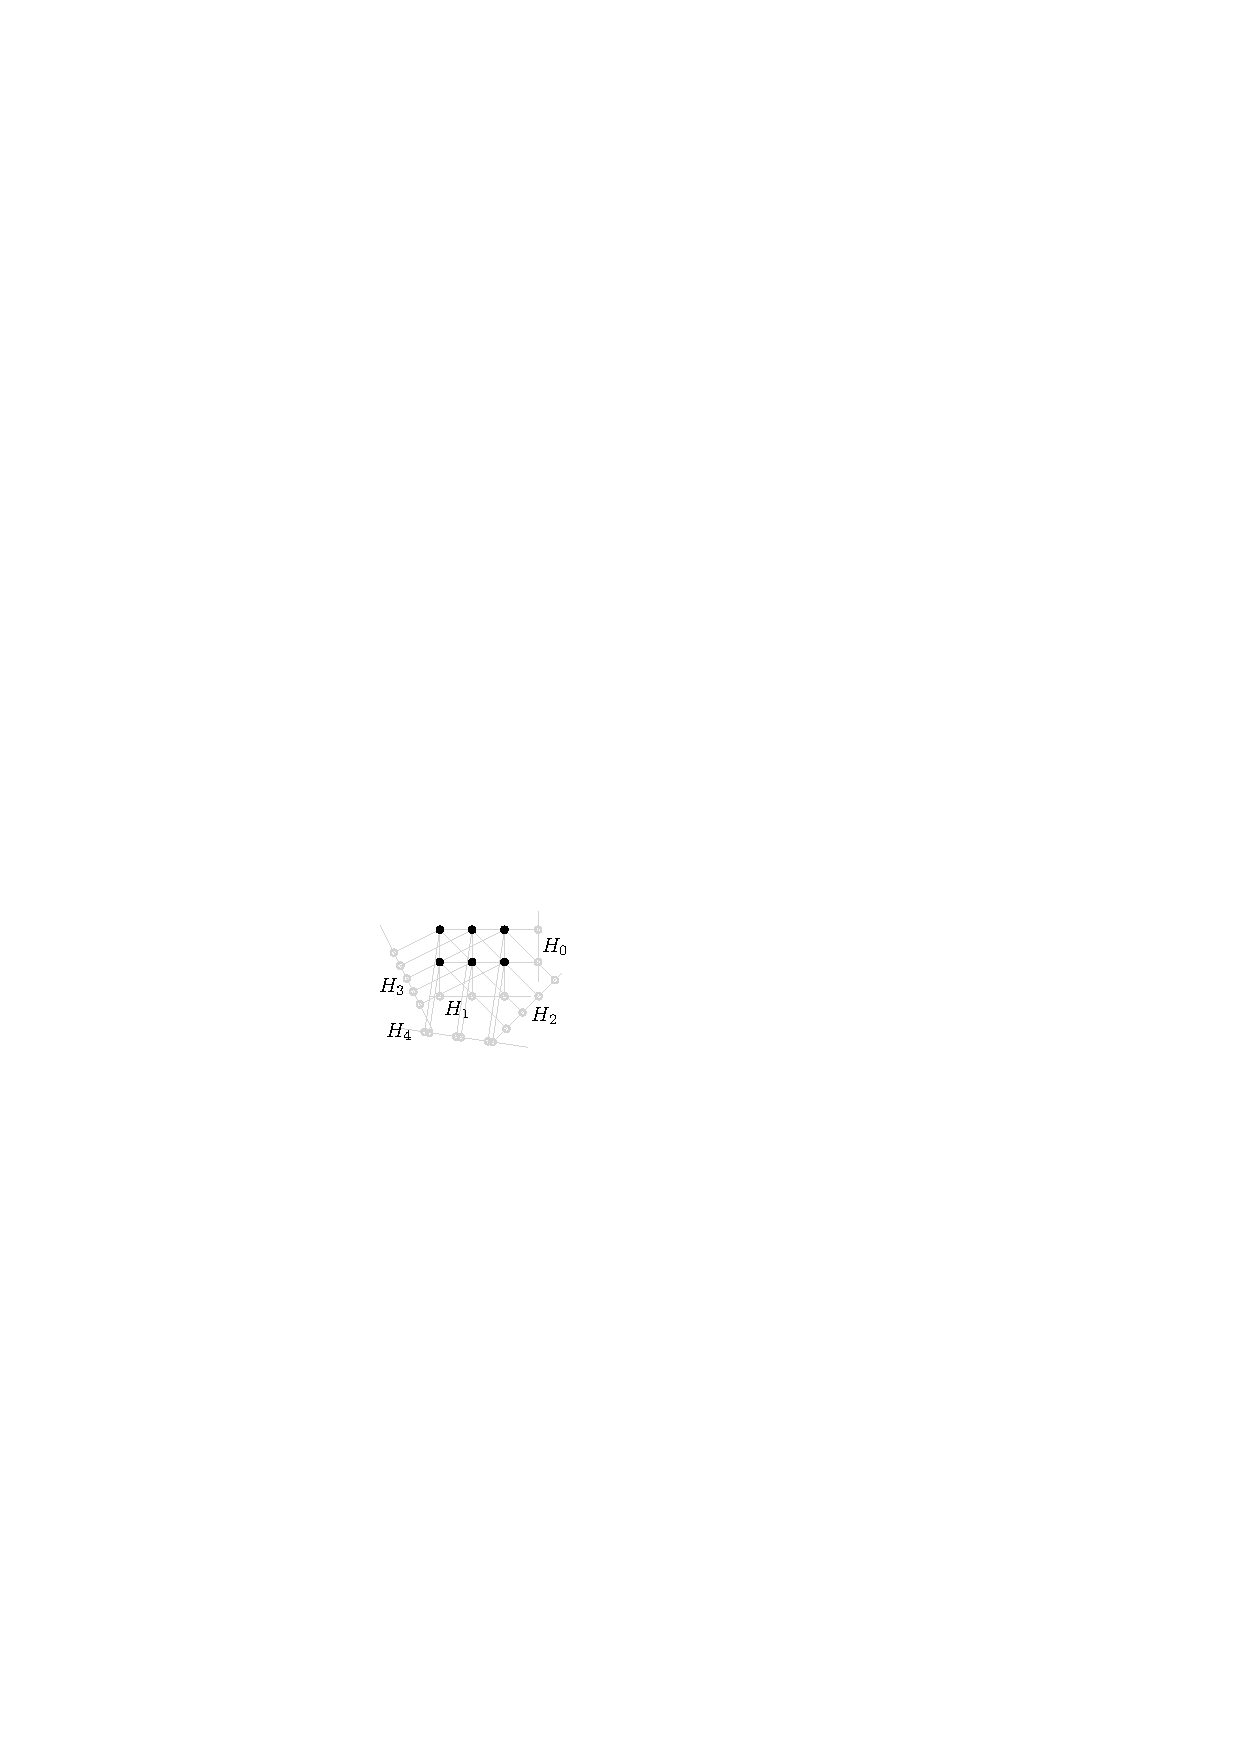
\includegraphics{i2.pdf} \\
%     \includegraphics[scale=1.2]{i1n.eps} \hspace{5mm} &  \hspace{5mm} 
%     \includegraphics[scale=0.8]{i2n.eps} \\
     (a) \hspace{5mm}  & \hspace{5mm}  (b)
  \end{tabular}
  \caption{Point sets showing that (a)~$t(1) \ge 2$ and (b)~$t(2) \ge 5$.}
  \label{fig:i1i2}
\end{figure}

Notice that the proof of Lemma \ref{lem:i1i2} implies that, for any $i$, 
$t(i)\le i^2 + 1$.  The following lemma shows that, for $i\ge 3$, $t(i)\le i^2$.  Of course, this upper bound is tighter than Lemma \ref{lem:upper-bound} for $i\le 123$.

\begin{lemma}\label{lem:i3}
$t(3)=9$.
\end{lemma}

\begin{proof}
The point set $S(4)$ described in the proof of Lemma \ref{lem:lower-bound}
results in 3 distinct points when they are projected onto a vertical line, therefore
$t(3)\ge 9$.

\begin{figure}[b]
  \begin{center}
    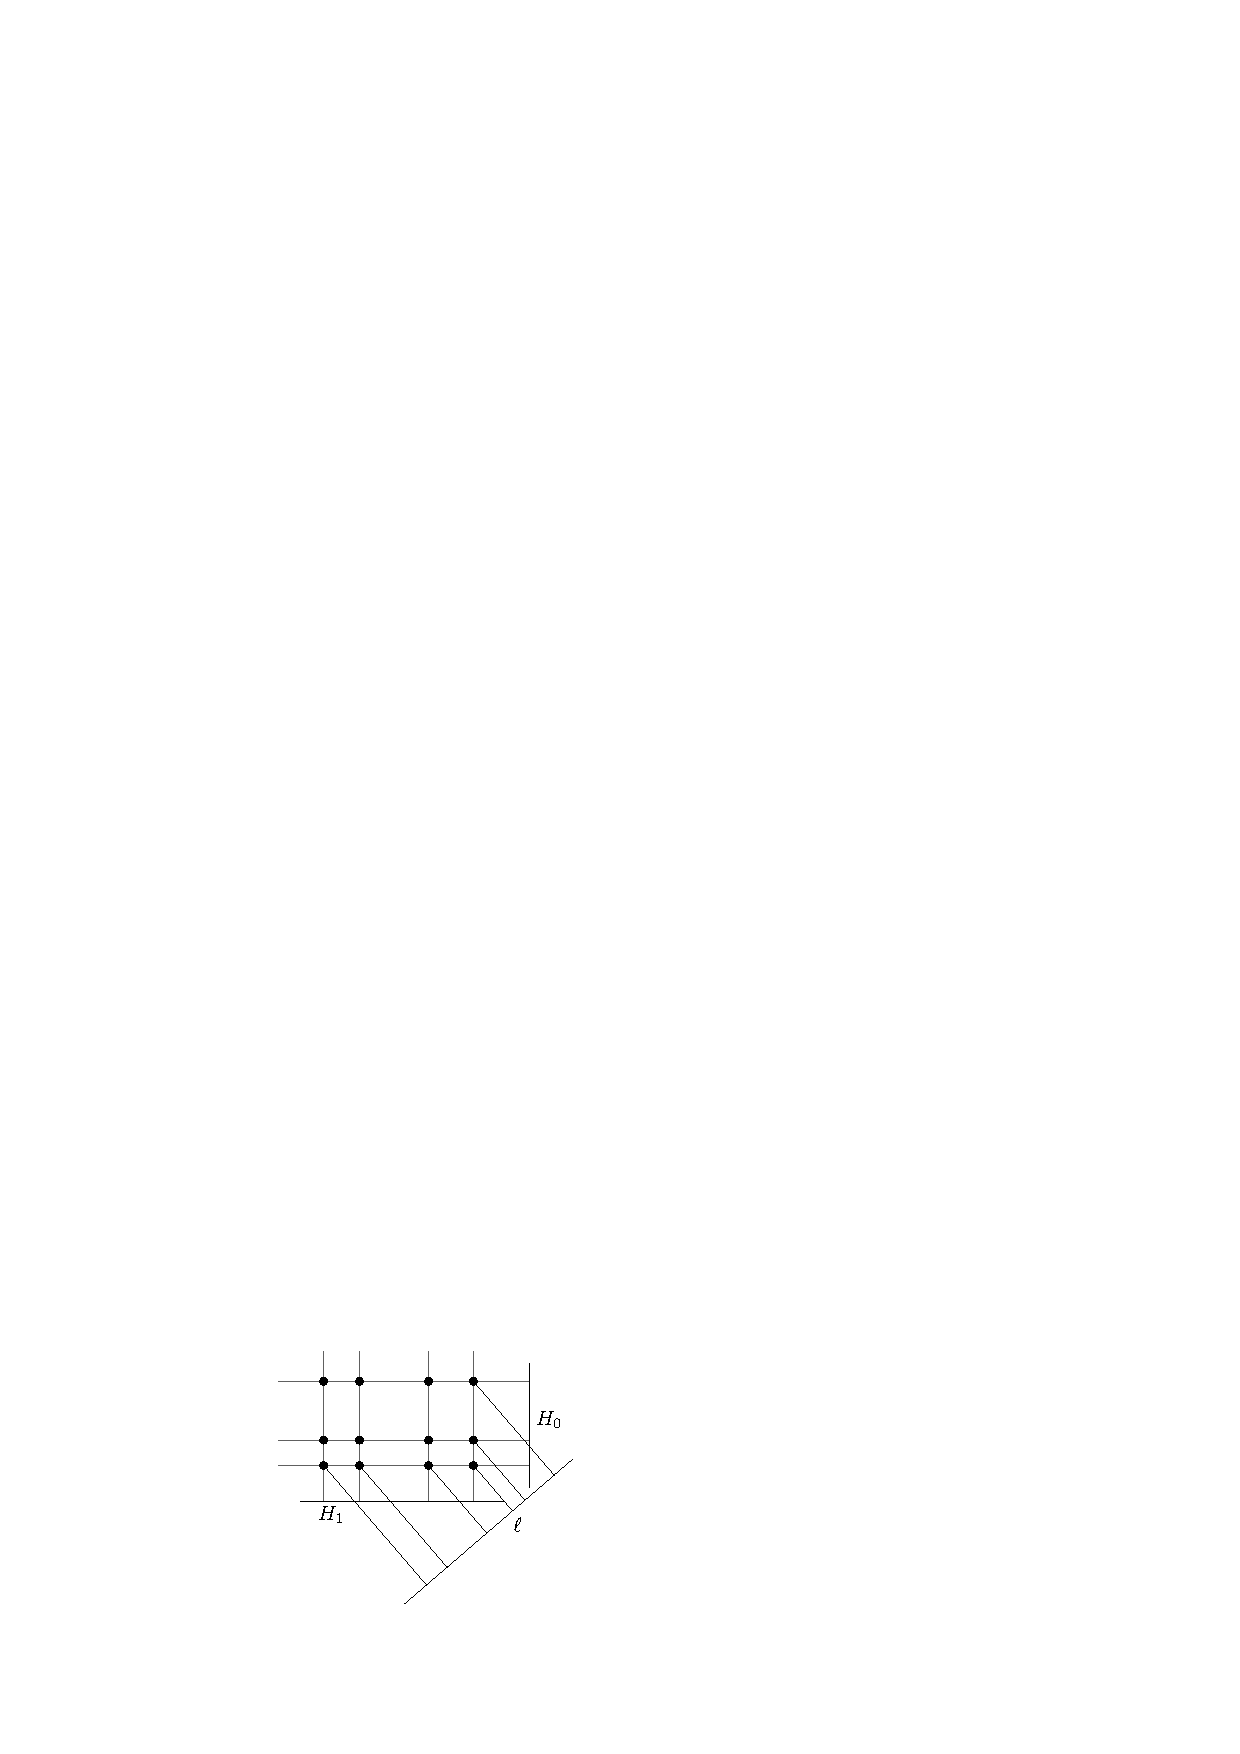
\includegraphics{3opt}
%    \includegraphics[bb=133 71 275 193]{3opt.ps}
%    \includegraphics[scale=0.7]{i3n.eps}
  \end{center}
  \caption{The proof of Lemma \ref{lem:i3}.}
  \label{fig:3opt}
\end{figure}

\begin{figure}
  \begin{center}
    \begin{tabular}{c@{}c}
       \hspace{-1cm}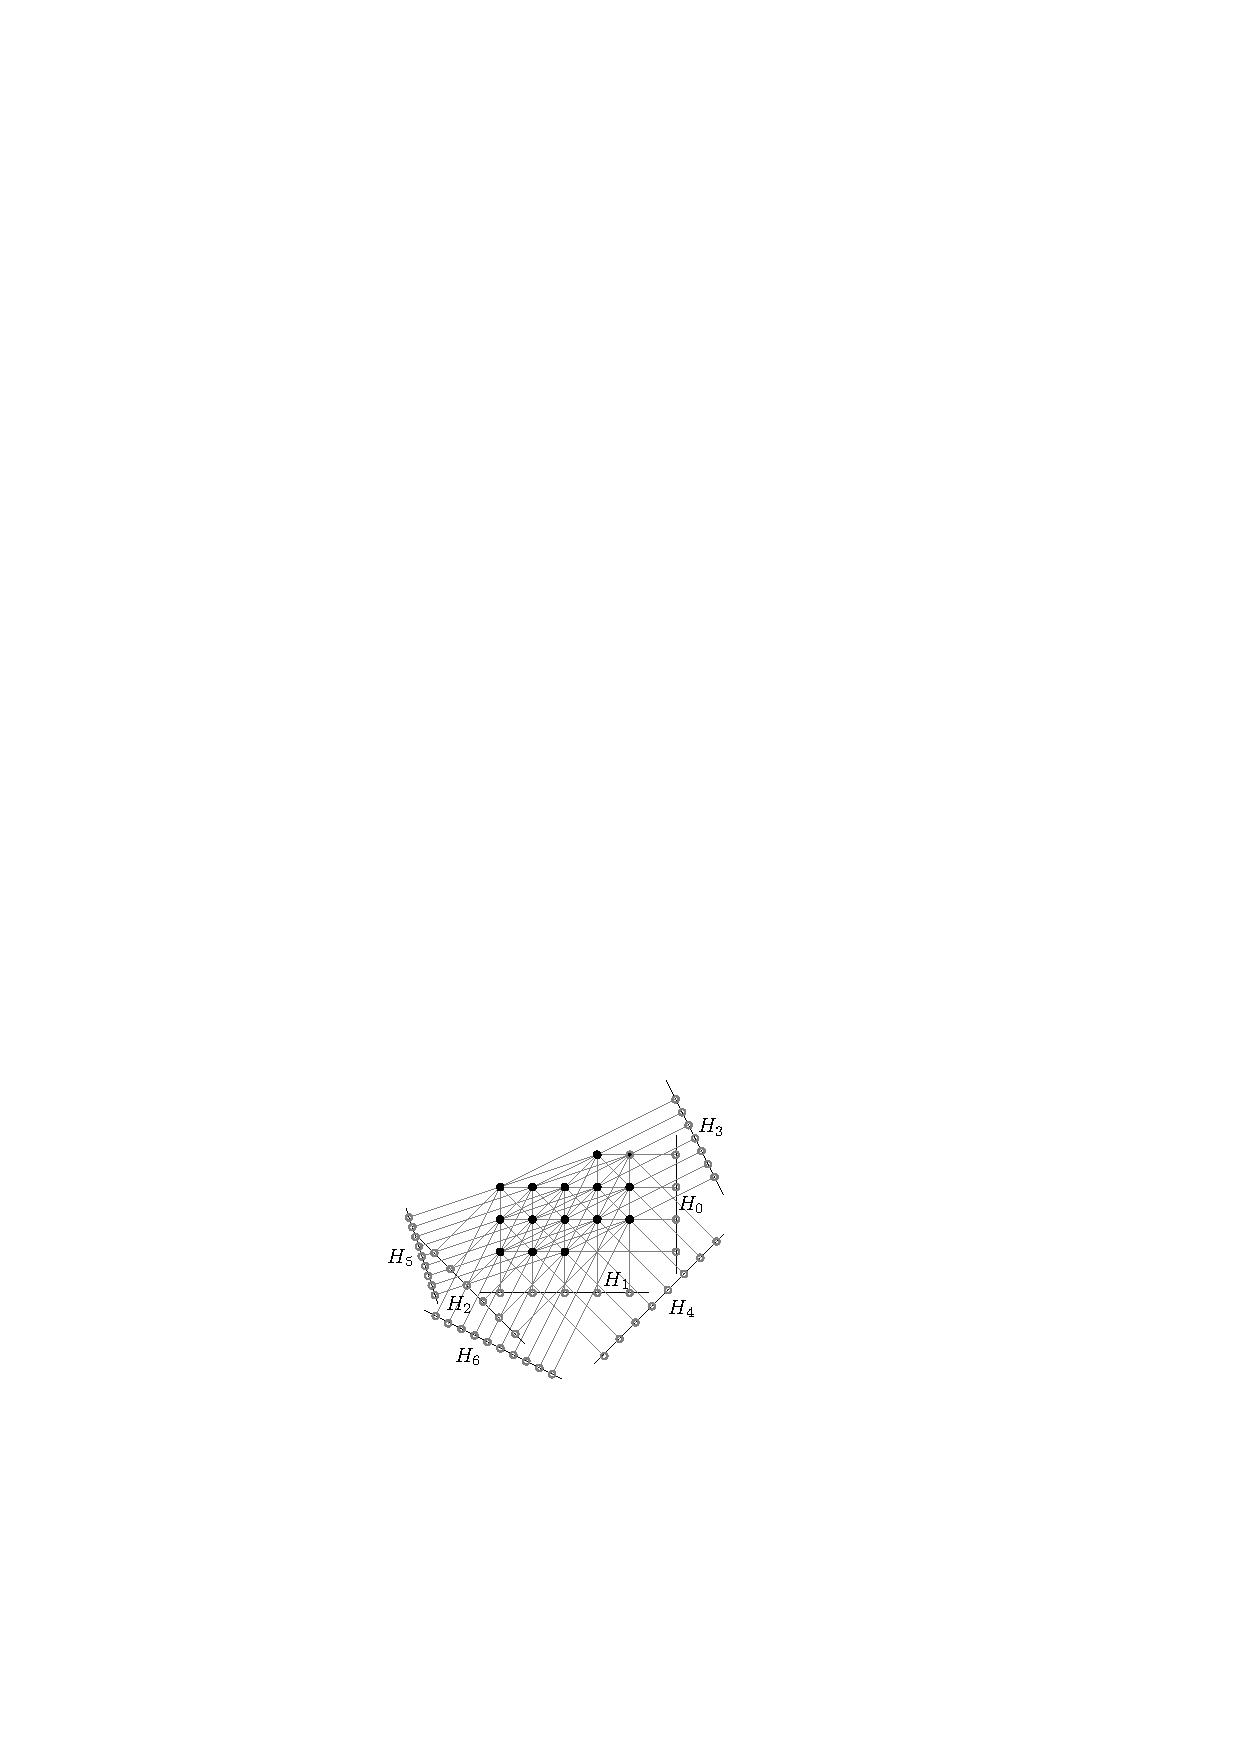
\includegraphics{i4a.pdf} & 
       \hspace{-1cm}
\includegraphics{i4b.pdf}
%      \includegraphics[width=0.54\linewidth]{i4a.ps} &
%      
\includegraphics[width=0.46\linewidth]{i4b.ps}
    \end{tabular}
  \end{center}
  \caption{A $(4,12)$ set of ghost chimneys.}
  \label{fig:i4}
\end{figure}

For the upper bound, refer to \figurename~\ref{fig:3opt}.  By an affine transformation,
we may assume that $H_0$ is vertical and $H_1$ is horizontal.  Thus, the
points of $S$ are contained in the intersection of 3 horizontal lines
with 4 vertical lines.  This establishes that $|S|\le 12$, so $t(3) \le 10$.
To see that $|S|< 12$, assume otherwise and consider any line $\ell$ that
is neither horizontal nor vertical. By a reflection through a horizontal
line, we may assume that $\ell$ has positive slope, so that every point
on the bottom row and right column of $S$ has a distinct projection
onto $\ell$, so $S$ projects onto at least 6 distinct points on $\ell$.
In particular, this implies that there is no line $H_2$ such that $S$
projects onto 5 distinct points on $H_2$.
\end{proof}

\begin{lemma}\label{lem:lower-bound-4}
$12 \le t(4) \le 15$.
\end{lemma}

\begin{proof}
The point set and lines $H_0,H_1,\ldots,H_{10}$ that show $t(4)\ge 12$
are shown in \figurename~\ref{fig:i4}.  ($H_{11}$ is omitted since any sufficiently
general line will do.)

To see that $t(4) \le 15$, we argue as in the proof of the second half
of Lemma \ref{lem:i3}.  This establishes that $|S|\le 20$.  If $|S|\in\{19,20\}$
then the number of distinct projections of $S$ onto $\ell$ is at least $7$,
but this contradicts the existence of $H_2$.  
Thus, we must have $|S|\le 18$, and hence $t(4)\le 15$.
\end{proof}


\section{Conclusions}

We have given upper and lower bounds on the largest possible value of $t$,
as a function of $i$, in an $(i,t)$ set of ghost chimneys.
These bounds differ by only an (admittedly large) constant factor.
Reducing this factor remains an open problem.
For small values of $i$, we have shown that $t(1)=2$, $t(2)=5$,
$t(3)=9$, and $12 \leq t(4) \leq 15$.

Another open problem is the generalization of these results to three,
or more, dimensions.  Given an integer $i$, what is the maximum
value $t(i)$ such that there exists a set of points $S\subset\R^d$
and a set $H_0,H_1,\ldots,H_{t(i)-1}$ of hyperplanes where, for each
$j\in\{0,1,\ldots,t(i)-1\}$, the orthogonal projection of $S$ onto $H_j$
consists of exactly $i+j$ distinct points?

%These ghost-chimney problems relate more generally to understanding
%what orthogonal projections a single 2D or 3D shape can have. In 2D
%closly related problems have been considered in \cite{Ski,
%mat}. Past explorations into structures in 3D, known variously as 3D
%ambigrams, trip-lets, and shadow sculptures, have focused on precise,
%usually connected projections \cite{triplets,ShadowArt}. Our work was
%originally motivated by considering what happens with disconnected projections of unspecified relative position.

\section*{Acknowledgments}

This work was initiated at the 25th Bellairs Winter Workshop on
Computational Geometry, co-organized by Erik Demaine and Godfried Toussaint,
held on February 6--12, 2010, in Holetown, Barbados.
We thank the other participants of that workshop 
%---Greg Aloupis, Brad Ballinger, Nadia Benbernou, Prosenjit Bose,
%S\'ebastien Collette, Mirela Damian, Karim Dou\"{\i}eb, Robin
%Flatland, Ferran Hurtado, John Iacono, Krishnam Raju Jampani, Anna
%Lubiw, Vera Sacristan, Stefan Langerman, Diane Souvaine---
 for providing a stimulating research environment.
The authors also thank to Adachi city for their permission to use
the photos including one in \figurename~\ref{fig:chimneys}.

% % Decrease the space between bibliography items.
% \let\realbibitem=\bibitem
% \def\bibitem{\par \vspace{-1.2ex}\realbibitem}

\bibliographystyle{unsrt}
\bibliography{chimneys}

\end{document}

\section{General Appearance}	%) A SECTION HEADING

Contributions to the {\it International Journal of Computational Geometry 
\& Applications} will be reproduced by photographing the author's
submitted typeset manuscript. It is therefore essential that the
manuscript be in its final form, and of good appearance because
it will be printed directly without any editing. The manuscript
should also be clean and unfolded. The copy should be evenly
printed on a high resolution printer (600 dots/inch or higher).
If typographical errors cannot be avoided, use cut and paste
methods to correct them. Smudged copy, pencil or ink text
corrections will not be accepted. Do not use cellophane or
transparent tape on the surface as this interferes with the
picture taken by the publisher's camera.

\section{The Main Text}

Contributions are to be in English. Authors are encouraged to
have their contribution checked for grammar. American spelling
should be used. Abbreviations are allowed but should be spelt
out in full when first used. Integers ten and below are to be
spelt out. Italicize foreign language phrases (e.g.~Latin,
French).

The text is to be typeset in 10 pt roman, single spaced
with baselineskip of 13~pt. Text area (including copyright block)  
is 8 inches high and 5 inches wide for the first page.  
Text area (excluding running title) is 7.7 inches high and 
5 inches wide for subsequent pages.  Final pagination and 
insertion of running titles will be done by the publisher.

\section{Major Headings}

Major headings should be typeset in boldface with the first
letter of important words capitalized.

\subsection{Sub-headings}

Sub-headings should be typeset in boldface italic and capitalize
the first letter of the first word only. Section number to be in
boldface roman.

\subsubsection{Sub-subheadings}

Typeset sub-subheadings in medium face italic and capitalize the
first letter of the first word only. Section numbers to be in
roman.

\subsection{Numbering and spacing}

Sections, sub-sections and sub-subsections are numbered in
Arabic.  Use double spacing before all section headings, and
single spacing after section headings. Flush left all paragraphs
that follow after section headings.

\subsection{Lists of items}

Lists may be laid out with each item marked by a dot:
\begin{itemlist}
 \item item one,
 \item item two.
\end{itemlist}
Items may also be numbered in lowercase roman numerals:
\begin{romanlist}
\item item one
\item item two 
	\begin{romanlist}[(b)]
	\item Lists within lists can be numbered with lowercase 
              roman letters,
	\item second item. 
	\end{romanlist}
\end{romanlist}

\section{Equations}

Displayed equations should be numbered consecutively,
with the number set flush right and enclosed in parentheses
\begin{equation}
\mu(n, t) = {\sum^\infty_{i=1} 1(d_i < t, N(d_i) 
= n)}{\int^t_{\sigma=0} 1(N(\sigma) = n)d\sigma}\,.
\label{eq:jaa}
\end{equation}

Equations should be referred to in abbreviated form,
e.g.~``Eq.~(\ref{eq:jaa})'' or ``(2)''. In multiple-line
equations, the number should be given on the last line.

Displayed equations are to be centered on the page width.
Standard English letters like x are to appear as $x$
(italicized) in the text if they are used as mathematical
symbols. Punctuation marks are used at the end of equations as
if they appeared directly in the text.

\section{Theorem environments}

\begin{theorem} \label{theo1}
Theorems, lemmas, etc. are to be numbered consecutively in the
paper. Use double spacing before and after theorems, lemmas, etc.
\end{theorem}

The labels cited in the theorem environments text can 
cross link to the body text e.g. Theorem~\ref{theo1} 
and Lemma~\ref{lemm1}.

\begin{lemma}  \label{lemm1}
Theorems, lemmas, etc. are to be numbered consecutively in the
paper. Use double spacing before and after theorems, lemmas, etc.
\end{lemma}

\begin{proof}
Proofs should end with
\end{proof}

\section{Illustrations and Photographs}

\begin{figure}[b]
\centerline{\psfig{file=ijcgaf1.eps,width=5cm}}
\vspace*{8pt}
\caption{A schematic illustration of dissociative recombination. The
direct mechanism, 4m$^2_\pi$ is initiated when the
molecular ion S$_{\rm L}$ captures an electron with 
kinetic energy. \label{fig1}}
\end{figure}

Figures are to be inserted in the text nearest their first
reference.  Figure~\ref{fig1} placements can be either top or 
bottom. Softcopies of illustrations are to be in either EPS, PS
or TIF format, preferably on a PC platform. Please prepare in 
300 dpi for line drawings (black and white); 
300 dpi for halftones (gray scale); 
300 dpi for colour images. Must be in CMYK (Cyan, Magenta,
Yellow and Black) for colour separation. If the author requires the
publisher to reduce the figures, ensure that the figures (including
letterings and numbers) are large enough to be clearly seen after
reduction. If photographs are to be used, only black and white ones 
are acceptable.

Figures are to be sequentially numbered in Arabic numerals. The
caption must be placed below the figure. Typeset in 8 pt roman
with baselineskip of 10~pt. Use double spacing between a
caption and the text that follows immediately.

Previously published material must be accompanied by written
permission from the author and publisher.

\section{Tables}

Tables should be inserted in the text as close to the point of
reference as possible. Some space should be left above and below
the table.

Tables should be numbered sequentially in the text in Arabic
numerals. Captions are to be centralized above the tables.
Typeset tables and captions in 8 pt roman with
baselineskip of 10 pt.

\begin{table}[h]
\tbl{Comparison of acoustic for frequencies for piston-cylinder problem.}
{\begin{tabular}{@{}cccc@{}} \toprule
Piston mass & Analytical frequency & TRIA6-$S_1$ model &
\% Error \\
& (Rad/s) & (Rad/s) \\ \colrule
1.0\hphantom{00} & \hphantom{0}281.0 & \hphantom{0}280.81 & 0.07 \\
0.1\hphantom{00} & \hphantom{0}876.0 & \hphantom{0}875.74 & 0.03 \\
0.01\hphantom{0} & 2441.0 & 2441.0\hphantom{0} & 0.0\hphantom{0} \\
0.001 & 4130.0 & 4129.3\hphantom{0} & 0.16\\ \botrule
\end{tabular}}
\begin{tabnote}
Table notes
\end{tabnote}
\end{table}

If tables need to extend over to a second page,
the continuation of the table should be preceded by a caption,
e.g.~``{\it Table 2.} $(${\it Continued}$)$''

\section{Running Heads}

Please provide a shortened runninghead (not more than eight words) for
the title of your paper. This will appear on the top right-hand side
of your paper.

\section{Footnotes}

Footnotes should be numbered sequentially in superscript
lowercase roman letters.\footnote{Footnotes should be
typeset in 8 pt roman at the bottom of the page.}

\section*{Acknowledgements}

This section should come before the References. Funding
information may also be included here.

\appendix

\section{Appendices}

Appendices should be used only when absolutely necessary. They
should come after the References. If there is more than one
appendix, number them alphabetically. Number displayed equations
occurring in the Appendix in this way, e.g.~(\ref{appeqn}), (A.2),
etc.
\begin{equation}
\mu(n, t) = {\sum^\infty_{i=1} 1(d_i < t, N(d_i) 
= n)}{\int^t_{\sigma=0} 1(N(\sigma) = n)d\sigma}\,.
\label{appeqn}
\end{equation}

\section*{References}

References are to be listed in the order cited in the text in Arabic
numerals.  They can be typed in superscripts after punctuation marks,
e.g.~``$\ldots$ in the statement.\cite{dolve}'' or used directly,
e.g.~``see Ref.~5 for examples.'' Please list using the style shown in
the following examples.  For journal names, use the standard
abbreviations.  Typeset references in 9 pt roman.

\begin{thebibliography}{0}
\bibitem{lorentz}
R. Lorentz and D. B. Benson, Deterministic and nondeterministic
flow-chart interpretations, {\it J. Comput. System Sci.}
{\bf 27} (1983) 400--433.

\bibitem{beeson}
M. J. Beeson, {\it Foundations of Constructive Mathematics}
(Springer, Berlin, 1985).

\bibitem{clark}
K. L. Clark, Negations as failure, in {\it Logic and Data
Bases}, eds. H. Gallaire and J.~Winker (Plenum Press, New York,
1973) 293--306.

\bibitem{joliat}
M. Joliat, A simple technique for partial elimination of unit
productions from LR({\it k}) parsers, {\it IEEE Trans.
Comput.} {\bf 27} (1976) 753--764.

\bibitem{dolve}
D. Dolve, Unanimity in an unknown and unreliable environment, in
{\it Proc. 22nd Annual Symp. Foundations of Computer
Science}, Nashville, TN (Oct. 1981) pp.~159--168.

\bibitem{tamassia}
R. Tamassia, C. Batini and M. Talamo, An algorithm for automatic
layout of entity relationship diagrams, in {\it
Entity-Relationship Approach to Software Engineering, Proc. 3rd
Int.  Conf. Entity-Relationship Approach}, eds. C. G. Davis,
S. Jajodia, P. A. Ng and R. T. Yeh (North-Holland, Amsterdam,
1983) pp.~421--439.

\bibitem{gewirtz}
W. L. Gewirtz, Investigations in the theory of descriptive
complexity, Ph. D. Thesis, New York University (1974).
\end{thebibliography}

\end{document}




